\documentclass[a4paper,11pt]{article}
\usepackage{amsmath}
\usepackage{indentfirst}
\usepackage{enumerate}
\usepackage{graphicx}
\usepackage{wrapfig}
\usepackage{amssymb}
\usepackage{float}
\usepackage{subfigure}
\usepackage{cite}
\usepackage{caption}
\usepackage{setspace}
\usepackage{fancyhdr}
\usepackage{lastpage}
\usepackage{layout}
\usepackage{geometry}
\usepackage{tikz,mathpazo}
\usepackage{pifont}
\usepackage[colorlinks,linkcolor=blue,anchorcolor=red,citecolor=green]{hyperref}
\usepackage{xcolor}
\usepackage{eso-pic}
\usepackage{extpfeil}
\usepackage[UTF8]{ctex}
\newtheorem{proof}{proof}[section]
\newtheorem{problem}{problem}[subsection]
\newtheorem{example}{example}[subsection]
\newtheorem{theorem}{theorem}[subsection]
\newcommand{\mG}{\mathcal{G}}
\begin{document}
\title{X.G.Wen Note}
\author{C.X.Lee\\\textit{Institute of physics, Chinese academy of sciences}}
\maketitle
\section{Functional differentiation}
The differentiation
\begin{equation*}
  F[f+\epsilon g]-F[f]=\epsilon\cdot DF_f[g]+O(\epsilon^2)
\end{equation*}
where the linear differential $DF_f$ is a linear functional.
\begin{equation*}
  DF_f[g_1+g_2]=DF_f[g_1]+DF_f[g_2]
\end{equation*}
A functional $F$ is said to be stationary of $f$, if only if $DF_f=0$. We need to Compute the differential $DF$.
\begin{equation*}
  F[f]\longrightarrow F(\mathbf{f})\quad\mathbf{f}=\{f_n\equiv f(x_n),n=1,2,\cdots,N\}
\end{equation*}
\begin{figure}[H]
  \centering
  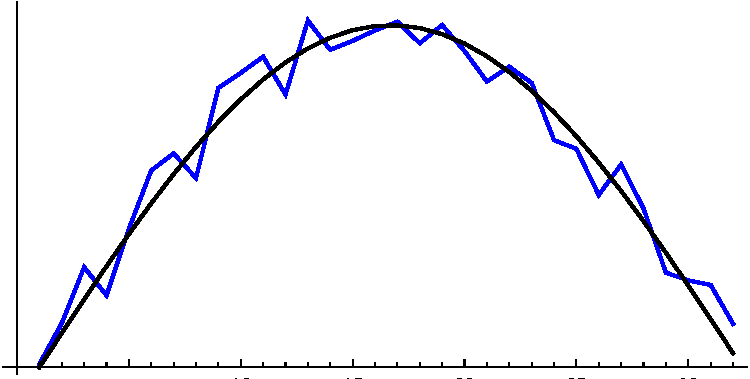
\includegraphics[width=3in]{1.pdf}
  \caption{Discrete vector $\mathbf{f}=\{f_n\equiv f(x_n),n=1,\cdots,N\}$}\label{fig1}
\end{figure}
\begin{equation*}
  \mathbf{f}\longleftrightarrow \text{N-dimensional vector space}
\end{equation*}
$F(\mathbf{f})$is a function defined over N-dimensional space.

The ordinary differential defined through
\begin{equation*}
  F(\mathbf{f}+\epsilon\mathbf{g})-F(\mathbf{f})=\epsilon\cdot dF_\mathbf{f}(g)+\mathcal{O}(\epsilon^2)
\end{equation*}
In a Cartesian Basis of $N$ unit vectors, $\mathbf{e}_n,\,n=1,\dots,N,\,dF_\mathbf{f}(\mathbf{g})\equiv\langle\nabla F_\mathbb{f},\mathbf{g}\rangle$
\begin{equation*}
  \langle\mathbf{f},\mathbf{g}\rangle=\sum_{n=1}^{N}f_ng_n\quad\nabla F_\mathbf{f}=\{\partial_{f_n}F\}
\end{equation*}
\begin{equation*}
  \partial_{f_n}F(\mathbf{f})=\lim_{\epsilon\to0}\frac{1}{\epsilon}[F(\mathbf{f}+\epsilon\mathbf{e}_n)-F(\mathbf{f})]
\end{equation*}
Thus
\begin{equation*}
  dF_{\mathbf{f}}(g)=\langle\nabla F_\mathbf{f},g\rangle=\sum_{n}\partial_{f_n}F(\mathbf{f})g_n
\end{equation*}
\begin{center}
  The limit $N\to\infty$, Discrete$\longrightarrow$ Continue
  \begin{equation*}
    \langle\mathbf{f},\mathbf{g}\rangle=\sum_{n}f_n,g_n\longmapsto\langle fg\rangle=\int dx f(x)g(x)
  \end{equation*}
\end{center}
The analog of the nth unit vector is a $\delta$-distribution, $\mathbf{e}_n\to\delta_x$, where $\delta_x(x')=\delta(x-x')$
\begin{equation*}
  f_n=\langle\mathbf{f},\mathbf{e}_n\rangle=\sum_{m}f_m(e_n)_m\to f(x)=\langle f,\delta_x\rangle=\int dx'f(x')\delta_x(x')
\end{equation*}
where $(e_n)_m=\delta_{nm}$
\begin{center}
  UNIT VECTOR$\longleftrightarrow\delta$ DISTRIBUTION
\end{center}
\begin{equation*}
  dF_\mathbf{f}(\mathbf{g})=\sum_{n}\partial_{f_n}F(\mathbf{f})g_n\longmapsto DF_f[g]=\int dx\frac{\delta F[f]}{\delta f(x)}g(x)
\end{equation*}
\begin{equation*}
  \frac{\delta F[f]}{\delta f(x)}=\lim_{\epsilon\to0}\frac{1}{\epsilon}\left(F[f+\epsilon\delta_x]-F[f]\right)
\end{equation*}
Chain rule
\begin{equation*}
  \frac{\delta F[g(f)]}{\delta f(x)}=\left.\int dy\frac{\delta F[g]}{g(y)}\right|_{g=g[f]}\frac{\delta g[f]}{\delta f(x)}
\end{equation*}
Talor series:
\begin{equation*}
  \begin{split}
     &\left.F[f]=F[\bar{f}]+\int dx_1\frac{\delta F[f]}{\delta f(x_1)}\right|_{f=\bar{f}}(f(x_1)-\bar{f}(x_1))+\\
       &\left.\frac{1}{2}\int dx_1dx_2\frac{\delta^2F[f]}{\delta f(x_1)\delta f(x_2)}\right|_{f=\bar{f}}(f(x_1)-\bar{f}(x_1))(f(x_2)-\bar{f}(x_2))+\cdots
  \end{split}
\end{equation*}
\section{Compute path integral}
\subsection{Discrete compute}
\begin{equation*}
  iG(x_b,t_b,x_a,t_a)=\int D[x(t)]e^{\frac{i}{\hbar}\int_{t_a}^{t_b}dtL(t,x,\dot{x})}=\int D[x(t)]e^{\frac{i}{\hbar}S(x_b,t_b,x_a,t_a)}
\end{equation*}
In semiclassical limit situation, $S\geq\hbar=1$. Phase $e^{iS}$ changes rapidly, and contributions from different paths cancel each other out.
\begin{equation*}
  \left.S[x_c(t)+\delta x(t)]=S[x_c(t)]+\int dt_1\frac{\delta S[x]}{\delta x(t_1)}\right|_{x=x_c}\delta x(t_1)+\left.\int dt_1dt_2\frac{\delta^2 S[x]}{\delta x(t_1)\delta x(t_2)}\right|_{x=x_c}\delta x(t_1)\delta x(t_2)+\cdots
\end{equation*}
Near the stable path $x_c(t)$
\begin{equation*}
  \left.\frac{\delta S}{\delta x(t)}\right|_{x=x_c}=0
\end{equation*}
\begin{equation*}
  S[x_c(t)+\delta x(t)]=S[x_c(t)]+\int dt_1dt_2\frac{\delta^2 S[x]}{\delta x(t_1)\delta x(t_2)}|_{x=x_c}\delta x(t_1)\delta x(t_2)
\end{equation*}
\begin{example}[Freedom particle]
  \begin{equation*}
    iG(x_b,t_b,x_a,t_a)=\left(\frac{m}{2\pi i\Delta t}\right)^{\frac{N}{2}}\int dx_1\cdots dx_{N-1}\prod_{j=1}^{N}exp\left\{i\frac{m}{2}\frac{(x_j-x_{j-1})^2}{\Delta t^2}\Delta t\right\}
  \end{equation*}
  Near the classical path
  \begin{equation*}
    x_c=x_a+\frac{x_b-x_a}{t_b-t_a}(t-t_a),\quad S_c=\int_{t_a}^{t_b}dtL=\frac{m(x_b-x_a)^2}{2(t_b-t_a)}
  \end{equation*}
  Consider the quantum fluctuation
  \begin{equation*}
    x_j=x_c(t_j)+\delta x_j,\quad t_j=t_a+j\Delta t
  \end{equation*}
  \begin{equation*}
    \begin{split}
       &iG(x_b,t_b,x_a,t_a)=\left(\frac{m}{2\pi i\Delta t}\right)^{\frac{N}{2}}\int dx_1\cdots dx_{N-1}\prod_{j=1}^{N}exp\left\{i\frac{m}{2\Delta
        t}(x_c(t_j)-x_c(t_{j-1})+\delta x_j-\delta x_{j-1})^2\right\}\\
         &=\left(\frac{m}{2\pi i\Delta t}\right)^{\frac{N}{2}}\int dx_1\cdots dx_{N-1}\prod_{j=1}^{N}exp\left\{i\frac{m}{2\Delta t}[(x_c(t_j)-x_c(t_{j-1}))^2\right.\\
         &\left.+2(x_c(t_j)-x_c(t_{j-1}))(\delta x_j-\delta x_{j-1})+(\delta x_j-\delta x_{j-1})^2]\right\}\\
         &=\left(\frac{m}{2\pi i\Delta t}\right)^{\frac{N}{2}}e^{iS_c}\int dx_1\cdots dx_{N-1}\prod_{j=1}^{N}exp{i\frac{m}{2\Delta t}[2(x_c(t_j)-x_c(t_{j-1}))(\delta x_j-\delta x_{j-1})+(\delta x_j-\delta x_{j-1})^2]}
    \end{split}
  \end{equation*}
  The first order term vanished
  \begin{equation*}
    \begin{split}
       iG(x_b,t_b,x_a,t_a)&=\left(\frac{m}{2\pi i\Delta t}\right)^{\frac{N}{2}}e^{iS_c}\int dx_1\cdots dx_{N-1}\prod_{j=1}^{N}exp\{i\frac{m}{2\Delta t}[(\delta x_j-\delta x_{j-1})^2]\}\\
         &=\left(\frac{m}{2\pi i\Delta t}\right)^{\frac{N}{2}}e^{iS_c}\int dx_1\cdots dx_{N-1}exp\{i\frac{m}{2\Delta t}\sum_{j=1}^{N}[\delta x_j^2+\delta x_{j-1}^2-2\delta x_j\delta x_{j-1}]\}\footnote{Boundary item $\delta x_0=\delta x_N=0$. The summary do not contain $j=0,j=N$ term.}\\
         &=\left(\frac{m}{2\pi i\Delta t}\right)^{\frac{N}{2}}e^{iS_c}\int dx_1\cdots dx_{N-1}exp\{i\sum_{jk=1}^{N-1}\delta x_jM_{jk}\delta x_k\}\\
         &=\left(\frac{m}{2\pi i\Delta t}\right)^{\frac{N}{2}}\sqrt{\frac{\pi^{N-1}}{Det(-iM)}}e^{iS_c}
    \end{split}
  \end{equation*}
  Boundary item $\delta x_0=\delta x_N=0$. The summary do not contain $j=0,j=N$ term. The sum can be take place $\sum_{j=1}^{N}\to\sum_{j,k=1}^{N-1}$
  \begin{equation*}
    M=\begin{bmatrix}
        2 & -1 & 0 & \cdots \\
        -1 & 2 & -1 & \cdots \\
        0 & -1 & 2 & \cdots \\
        \cdots & \cdots & \cdots & \cdots
      \end{bmatrix}
  \end{equation*}
\end{example}
For general quadratic Lagrangian
\begin{equation*}
  L=\frac{1}{2}m\dot{x}^2+b(t)x(t)\dot{x}(t)-\frac{1}{2}c(t)x^2(t)-e(t)x(t)
\end{equation*}
\begin{equation*}
  iG(x_b,t_b,x_a,t_a)=\int D[x(t)]e^{\frac{i}{\hbar}\int_{t_a}^{t_b}dt L}
\end{equation*}
Bound condition:
\begin{equation*}
  \begin{cases}
  x(t_a)=x_a,&\\
  x(t_b)=x_b,&.
  \end{cases}
\end{equation*}
Define fluctuation
\begin{equation*}
  y(\tau)=x(\tau)-\bar{x}(\tau)
\end{equation*}
\begin{equation*}
  \int_{t_a}^{t_b}d\tau L=S[x(\tau)]=S[\bar{x}(\tau)+y(\tau)]=S[\bar{x}]+\frac{1}{2}\int_{t_a}^{t_b}d\tau d\tau'y(\tau')\frac{\delta^2S}{\delta x(\tau')\delta x(\tau)}|_{x=\bar{x}}y(\tau)
\end{equation*}
Now compute the action of quadratic Lagrangian
\begin{equation*}
  S=\int_{t_a}^{t_b}dt\frac{1}{2}m\dot{x}^2+b(t)x\dot{x}-\frac{1}{2}c(t)x^2-e(t)x(t)
\end{equation*}
Take variation
\begin{equation*}
  \begin{split}
     \frac{\delta S}{\delta x(\tau)}=&\int_{t_a}^{t_b}dtm\dot{x}\frac{d}{dt}\delta(t-\tau)+b(t)\delta(t-\tau)\dot{x}+b(t)x(t)\frac{d}{dt}\delta(t-\tau)-c(t)x(t)\delta(t-\tau)-e\delta(t-\tau)\\
       &=-m\ddot{x}(\tau)+b\dot{x}\delta(t-\tau)-b\dot{x}(\tau)-cx(\tau)-e
  \end{split}
\end{equation*}
\begin{equation*}
  \frac{\delta^2 S}{\delta x(\tau')\delta x(\tau)}=-m\frac{d^2}{d\tau^2}\delta(\tau'-\tau)-c\delta(\tau'-\tau)
\end{equation*}
Thus
\begin{equation*}
  \begin{split}
     &\frac{1}{2}\int d\tau d\tau'y(\tau')\frac{\delta^2S}{\delta x(\tau')\delta x(\tau)}|_{x=\bar{x}}y(\tau)\\
       &=\frac{1}{2}\int d\tau d\tau'y(\tau')\left[-m\frac{d^2}{d\tau^2}\delta(\tau'-\tau)-c\delta(\tau'-\tau)\right]|_{x=\bar{x}}y(\tau)\\
       &=-\frac{1}{2}\int d\tau y(\tau)(m\frac{d^2}{d\tau^2}+c(t))y(\tau)\\
       &=\int d\tau(\frac{m}{2}\dot{y}^2-\frac{1}{2}cy^2)
  \end{split}
\end{equation*}
\begin{equation*}
  iG(x_b,t_b,x_a,t_a)=\int D[x]e^{\frac{i}{\hbar}\int_{t_a}^{t_b}d\tau L}=e^{\frac{i}{\hbar}S_c}\int D[y]e^{\frac{i}{\hbar}\int dt(\frac{m}{2}\dot{y}^2-\frac{c}{2}y^2)}
\end{equation*}
Discrete and define $i\tilde{G}(0,t_b,0,t_a)=\int D[y]e^{\frac{i}{\hbar}\int dt(\frac{m}{2}\dot{y}^2-\frac{c}{2}y^2)}$
\begin{equation*}
  i\tilde{G}(0,t_b,0,t_a)=\lim_{N\to\infty}\left(\frac{m}{2\pi i\hbar\Delta t}\right)^{\frac{N}{2}}\int dy_1\cdots dy_{N-1}exp\left[\frac{i}{\hbar}\sum_{j=1}^{N}\left(\frac{m}{2\Delta t}(y_j-y_{j-1})^2-\frac{\Delta t}{2}c_jy_j^2\right)\right]
\end{equation*}
where $c_j=c(t_j),\,t_j=t_a+j\Delta t$. Define $\eta=\begin{bmatrix}
                                                       y_1 \\
                                                       \vdots \\
                                                       y_{N-1}
                                                     \end{bmatrix}$
\begin{equation*}
  i\tilde{G}(0,t_b,0,t_a)=\lim_{N\to\infty}\left(\frac{m}{2\pi i\hbar\Delta t}\right)^{\frac{N}{2}}\int d\eta e^{-\eta^T\sigma\eta}
\end{equation*}
where $\sigma=\frac{m}{2i\hbar\Delta t}\begin{bmatrix}
                2 & -1 & \quad & \quad & \quad & \quad \\
                -1 & 2 & -1 & \quad & \quad & \quad \\
                \quad & -1 & 2 & \ddots & \quad & \quad \\
                \quad & \quad & \ddots & \ddots & \quad & \quad \\
                \quad & \quad & \quad & \quad & 2 & -1 \\
                \quad & \quad & \quad & \quad & -1 & 2
              \end{bmatrix}+\frac{i\Delta t}{2\hbar}\begin{bmatrix}
                                                       c_1 & \quad & \quad & \quad & \quad & \quad \\
                                                       \quad & c_2 & \quad & \quad & \quad & \quad \\
                                                       \quad & \quad & \ddots & \quad & \quad & \quad \\
                                                       \quad & \quad & \quad & \ddots & \quad & \quad \\
                                                       \quad & \quad & \quad & \quad & c_{N-2} & \quad \\
                                                       \quad & \quad & \quad & \quad & \quad & c_{N-1}
                                                     \end{bmatrix}$
$\sigma=i\tilde{\sigma}$, $\tilde{\sigma}$ is Hermitian. $\sigma=U^\dag\sigma_DU$. $Det(\sigma_D)=1$
\begin{equation*}
  \begin{split}
     i\tilde{G}(0,t_b,0,t_a)&=\lim_{N\to\infty}\left(\frac{m}{2\pi i\hbar\Delta t}\right)^{\frac{N}{2}}\sqrt{\frac{\pi^{N-1}}{Det\sigma}}\\
       &=\lim_{N\to\infty}\sqrt{\frac{m}{2\pi i\hbar\Delta t}\frac{1}{\left(\frac{2i\hbar\Delta t}{m}\right)^{N-1}Det\sigma}}
  \end{split}
\end{equation*}
\begin{equation*}
  \begin{split}
     &\left(\frac{2i\hbar\Delta t}{m}\right)^{N-1}Det\sigma=Det\left(\frac{2i\hbar\Delta t}{m}\sigma\right)\\
       &=Det\left(\begin{bmatrix}
                2 & -1 & \quad & \quad & \quad & \quad \\
                -1 & 2 & -1 & \quad & \quad & \quad \\
                \quad & -1 & 2 & \ddots & \quad & \quad \\
                \quad & \quad & \ddots & \ddots & \quad & \quad \\
                \quad & \quad & \quad & \quad & 2 & -1 \\
                \quad & \quad & \quad & \quad & -1 & 2
              \end{bmatrix}-\frac{\Delta t^2}{m}\begin{bmatrix}
                                                       c_1 & \quad & \quad & \quad & \quad & \quad \\
                                                       \quad & c_2 & \quad & \quad & \quad & \quad \\
                                                       \quad & \quad & \ddots & \quad & \quad & \quad \\
                                                       \quad & \quad & \quad & \ddots & \quad & \quad \\
                                                       \quad & \quad & \quad & \quad & c_{N-2} & \quad \\
                                                       \quad & \quad & \quad & \quad & \quad & c_{N-1}
                                                     \end{bmatrix}\right)\\
                                                     &=p_{N-1}
  \end{split}
\end{equation*}
\begin{equation*}
  p_j=Det\left\{\begin{bmatrix}
                  2-\frac{\Delta t^2}{m}c_1 & -1 & \quad & \quad & \quad \\
                  -1 & 2-\frac{\Delta t^2}{m}c_2 & \quad & \quad & \quad \\
                  \quad & \quad & \ddots & \quad & \quad \\
                  \quad & \quad & \quad & 2-\frac{\Delta t^2}{m}c_{j-1} & -1 \\
                  \quad & \quad & \quad & -1 & 2-\frac{\Delta t^2}{m}c_j
                \end{bmatrix}\right\}
\end{equation*}
Laplace expansion
\begin{equation*}
  p_{j+1}=(2-\frac{\Delta t^2}{m}c_{j+1})p_{j}-p_{j-1}
\end{equation*}
\begin{equation*}
  p_1=2-\frac{\Delta t^2}{m}c_1
\end{equation*}
\begin{equation*}
  \begin{split}
     p_{j+1}-2p_j+p_{j-1}&=-\frac{\Delta t^2}{m}c_{j+1}p_j\\
       \frac{p_{j+1-2p_j+p_{j-1}}}{\Delta t^2}&=-\frac{c_{j+1}p_j}{m}
  \end{split}
\end{equation*}
Define
\begin{equation*}
  \varphi(t_j)=\Delta p_j
\end{equation*}
\begin{equation*}
  \frac{d^2\varphi(t)}{dt^2}=-\frac{c(t)}{m}\varphi(t)
\end{equation*}
Notice that third-order determinant is $1$. $p_0=1$
\begin{equation*}
  \varphi(t_0)=\Delta tp_0\to 0
\end{equation*}
\begin{equation*}
  \frac{d\varphi(t)}{dt}=\lim_{\Delta t\to0}\frac{\varphi(t_1)-\varphi(t_0)}{\Delta t}=\lim_{\Delta t\to 0}(p_1-p_0)=\lim_{\Delta t\to 0}(1-\frac{\Delta t^2}{m}c_1)\to 1
\end{equation*}
Hence we can define that
\begin{equation*}
  f(t,t_a)=\varphi(t),\quad f(t_b,t_a)=\varphi(t_b),\quad f(t_a,t_a)=\varphi(t_a)=0,\quad \left.\frac{\partial f(t,t_a)}{\partial t}\right|_{t=t_a}=1
\end{equation*}
\begin{equation*}
  m\frac{\partial^2f(t,t_a)}{\partial t^2}+c(t)f(t,t_a)=0
\end{equation*}
\begin{equation*}
  \begin{split}
     iG(x_b,t_b,x_a,t_a)&=exp\left[\frac{i}{\hbar}S_c(x_b,t_b,x_a,t_a)\lim_{N\to\infty}\sqrt{\frac{m}{2\pi i\Delta t}\frac{1}{(\frac{2i\hbar\Delta t}{m})^{N-1}Det\sigma}}\right]\\
       &=exp\left[\frac{i}{\hbar}S_c(x_b,t_b,x_a,t_a)\lim_{N\to\infty}\sqrt{\frac{m}{2\pi i\Delta t}\frac{1}{p_{N-1}}}\right]\\
       &=e^{\frac{i}{\hbar}S_c}\sqrt{\frac{m}{2\pi i\hbar f(t_b,t_a)}}
  \end{split}
\end{equation*}
\begin{example}
  Harmonic oscillator $L=\frac{m}{2}\dot{x}^2-bx-\frac{m}{x}\omega^2x^2$
\end{example}
\begin{equation*}
  iG(x_b,t_b,x_a,t_a)=e^{iS_c}\sqrt{\frac{m}{2\pi i\hbar f(t_b,t_a)}}
\end{equation*}
\begin{equation*}
  m\frac{\partial^2f(t,t_a)}{\partial t^2}+m\omega f(t,t_a)=0
\end{equation*}
\begin{equation*}
  f(t,t_a)=A\cos\omega t+B\sin\omega t,\quad f(t_a,t_a)=0,\quad \left.\frac{\partial f(t,t_a)}{\partial t}\right|_{t=t_a}=1
\end{equation*}
\begin{equation*}
  f(t_b,t_a)=\frac{\sin\omega(t_b-t_a)}{\omega}
\end{equation*}
\begin{equation*}
  iG(x_b,t_b,x_a,t_a)=\sqrt{\frac{m\omega}{2\pi i\hbar\sin\omega(t_b-t_a)}}e^{iS_c}
\end{equation*}
\subsection{Continue compute}
\begin{figure}[H]
  \centering
  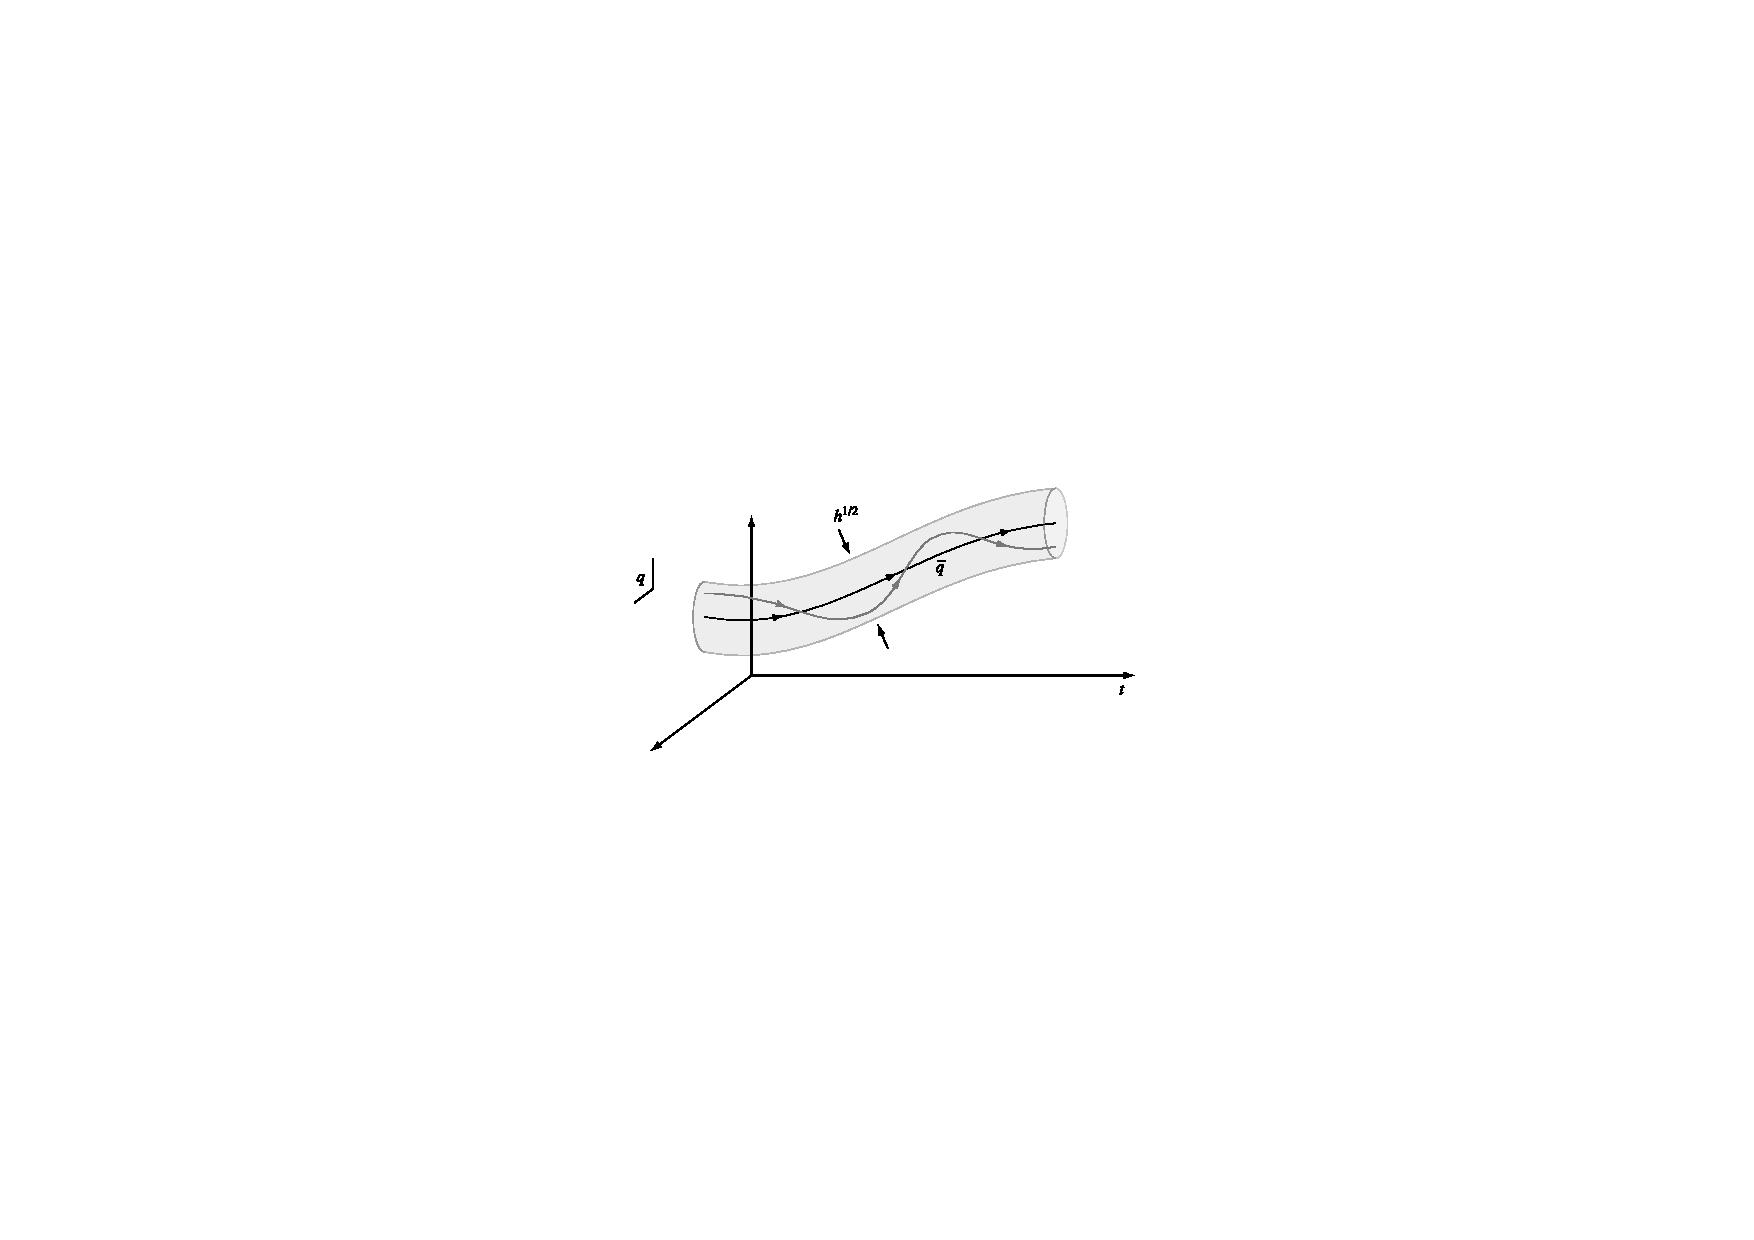
\includegraphics[width=4in]{2.pdf}
  \caption{Figure 2}
\end{figure}
Firstly we compute the Gaussian integral $\int Dx e^{-F[x]}$.
\begin{enumerate}
  \item Find the stationary phase point $\bar{x}$
  \begin{equation*}
    DF_x=0\Leftrightarrow\forall t:\left.\frac{\delta F[x]}{\delta x(t)}\right|_{x=\bar{x}}=0
  \end{equation*}
  Maybe there are some stationary phase configuration $\bar{x}_1,\dots,\bar{x}_s$. But here we only discuss the case in which the $\bar{x}$ is unique.
  \item Taylor series:
  \begin{equation*}
    F[x]=F[\bar{x}+y]=F[\bar{x}]+\frac{1}{2}\int dtdt' y(t')A(t,t')y(t)+\cdots
  \end{equation*}
  where the $A(t,t')=\frac{\delta^2 S}{\delta x(t)\delta x(t')}|_{x=\bar{x}}$. First order term is vanished.
  \item The operator $\hat{A}={A(t,t')}$ must be positive define.
  \begin{equation*}
    \int Dxe^{-F[x]}\simeq \sqrt{\frac{2\pi}{Det(A)}}e^{-F[\bar{x}]}
  \end{equation*}
  \item If there are many stationary phase configurations, $\bar{x}_i$, the individual contributions have to be added
  \begin{equation*}
    \int Dxe^{-F[x]}\simeq\sum_{i}e^{-F[\bar{x}_i]}\sqrt{Det\left(\frac{\hat{A}_i}{2\pi}\right)}
  \end{equation*}
\end{enumerate}
The fluctuation
\begin{equation*}
  r(t)=q(t)-q_{c}(t)
\end{equation*}
\begin{equation*}
  \langle q_f|e^{-\frac{i}{\hbar}Ht}|q_{i}\rangle\simeq e^{\frac{i}{\hbar}S_c}\int_{r(0)=r(t)=0}Drexp\left[\left.\frac{1}{2}\frac{i}{\hbar}\int_{0}^{t}dt'dt''r(t')\frac{\delta^2S[q]}{\delta q(t')\delta q(t'')}\right|_{q=q_c}r(t'')\right]
\end{equation*}
Compute $\frac{\delta^2 S}{\delta q(t)\delta q(t')}$
\begin{equation*}
  \begin{split}
      &=\frac{1}{2}\int_{0}^{t}dtdt'r(t)\left.\frac{\delta^2S[q]}{\delta q(t)\delta q(t')}\right|_{q=q_c}r(t')\\
       &=\frac{1}{2}\int_{0}^{t}dtdt'r(t)\left.\frac{\delta}{\delta q(t')}\frac{\delta S[q]}{\delta q(t)}\right|_{q=q_c}r(t')\\
       &=\frac{1}{2}\int_{0}^{t}dtdt'r(t)\left.\frac{\delta}{\delta q(t')}\frac{\delta}{\delta q(t)}\int d\tau[\frac{m}{2}\dot{q}^2(\tau)-V(\tau)]\right|_{q=q_c}r(t')\\
       &=\frac{1}{2}\int_{0}^{t}dtdt'r(t)\left.\frac{\delta}{\delta q(t')}\int d\tau\left[\frac{m}{2}2\dot{q}\frac{\delta}{\delta q(t)}\frac{d}{d\tau}q(\tau)-\frac{\partial V}{\partial q(\tau)}\frac{\delta q(\tau)}{\delta q(t)}\right]\right|_{q=q_c}r(t')\\
       &=\frac{1}{2}\int_{0}^{t}dtdt'r(t)\left.\frac{\delta}{\delta q(t')}\int d\tau\left[m\dot{q}\frac{d}{d\tau}\delta(t-\tau)-\frac{\partial V}{\partial q(\tau)}\delta(\tau-t)\right]\right|_{q=q_c}r(t')\\
       &=\frac{1}{2}\int_{0}^{t}dtdt'r(t)\left.\frac{\delta}{\delta q(t')}\left(-m\ddot{q}(t)-\frac{\partial V}{\partial q(t)}\right)\right|_{q=q_c}r(t')\\
       &=\frac{1}{2}\int_{0}^{t}dtdt'r(t)\left.\left(-m\frac{d^2}{dt^2}\delta(t-t')-\frac{\partial^2V}{\partial q(t')\partial q(t)}\delta(t-t')\right)\right|_{q=q_c}r(t')\\
       &=-\frac{1}{2}\int_{0}^{t}dtdt'r(t)\left.m\frac{d^2}{dt^2}\delta(t-t')\right|_{q=q_c}r(t')-\frac{1}{2}\int_{0}^{t}dtdt'\left.r(t)\frac{\partial^2V}{\partial q(t')\partial q(t)}\delta(t-t')\right|_{q=q_c}r(t')\\
       &=-\frac{1}{2}\int_{0}^{t}dtdt'm\frac{d^2}{dt^2}\left(r(t')r(t)\right)\delta(t-t')-\frac{1}{2}\int_{0}^{t}dtdt'\frac{d^2}{dt^2}\frac{\partial^2V}{\partial q(t')\partial q(t)}\delta(t-t')\\
       &=-\frac{1}{2}\int_{0}^{t}dtdt'mr(t')\ddot{r}(t)\delta(t-t')-\frac{1}{2}\int_{0}^{t}dtdt'\frac{d^2}{dt^2}\frac{\partial^2V}{\partial q(t')\partial q(t)}\delta(t-t')\\
       &=-\frac{1}{2}\int_{0}^{t}dtr(t)[m\partial_t^2+V''(q_{c}(t))]r(t)
  \end{split}
\end{equation*}

\section{Linear response}
\subsection{Formula 2.2.9}
\begin{equation*}
  iG_{x}(t_b,t_a)=\frac{\langle\psi|U^{\theta}(\infty,t_b)xU^\theta(t_b,t_a)xU^\theta(t_a,-\infty)|\psi\rangle}{\langle\psi|U^\theta(\infty,-\infty)|\psi\rangle}
\end{equation*}
The path integral
\begin{equation*}
  iG_x(t_b,t_a)=\frac{\int D[x(t)] x(t_b)x(t_a)e^{i\int_{-\infty}^{\infty}dt L}}{\int D[x(t)]e^{i\int_{-\infty}^{\infty}dt L}}
\end{equation*}
\begin{proof}
  \begin{equation*}
    -\infty\longmapsto t_a\longmapsto t_b\longmapsto\infty
  \end{equation*}
  \begin{equation*}
    x(t_b)=U^\dag(t_b,t_0)x(t_0)U(t_b,t_0)
  \end{equation*}
  \begin{equation*}
    x(t_a)=U^\dag(t_a,t_0)x(t_0)U(t_a,t_0)
  \end{equation*}
  Transform from Schrodinger picture to Heisenberg picture
  \begin{equation*}
    \begin{split}
       iG_{x}(t_b,t_a)&=\frac{\langle\psi|U^{\theta}(\infty,t_b)x(t_0)U^\theta(t_b,t_a)x(t_0)U^\theta(t_a,-\infty)|\psi\rangle}{\langle\psi|U^\theta(\infty,-\infty)|\psi\rangle}\\
         &=\frac{\langle\psi|U^{\theta}(\infty,t_b)U^\theta(t_b,t_0)xU^{\theta\dag}(t_b,t_0)U^\theta(t_b,t_a)U^\theta(t_a,t_0)x(t_a)U^{\theta\dag}(t_a,t_0)U^\theta(t_a,-\infty)|\psi\rangle}{\langle\psi|U^\theta(\infty,-\infty)|\psi\rangle}\\
         &=\frac{\langle\psi|U^\theta(\infty,t_0)x(t_b)x(t_a)U(t_0,-\infty)|\psi\rangle}{\langle\psi|U^\theta(\infty,-\infty)|\psi\rangle}\\
         &=\frac{\langle\psi(t_0)|x(t_b)x(t_a)|\psi(t_0)\rangle}{\langle\psi|U^\theta(\infty,-\infty)|\psi\rangle}\\
         &=\langle x(t_b)x(t_a)\rangle
    \end{split}
  \end{equation*}
  Define $\langle x|\psi\rangle=\delta(x)$\\
  \begin{equation*}
    iG_x(t_b,t_a)=\frac{\int dxdx'\langle\psi|x\rangle\langle x|U^\theta(\infty,t_b)x(t_b)U^\theta(t_b,t_a)x(t_a)U^\theta(t_a,-\infty)|x'\rangle\langle x'|\psi\rangle}{\langle\psi|U^\theta(\infty,-\infty)|\psi\rangle}
  \end{equation*}
  Using Delta function, the following formula can be derivated\\
  \begin{equation*}
    iG_x(t_b,t_a)=\frac{\langle x|U^\theta(\infty,t_b)x(t_b)U^\theta(t_b,t_a)x(t_a)U^\theta(t_a,-\infty)|x\rangle}{\langle x|U^\theta(\infty,-\infty)|x\rangle}
  \end{equation*}
  Insert$\int D[x(t_a)]|x(t_a)\rangle\langle x(t_a)|=1$,$\int D[x(t_b)]|x(t_b)\rangle\langle x(t_b)|=1$
  \begin{equation*}
    \begin{split}
       iG_x(t_b,t_a)&=\frac{\int D[x(t_a)]D[x(t_b)]x(t_a)x(t_b)\langle x|U^\theta(\infty,t_b)|x(t_b)\rangle\langle x(t_b)|U^\theta(t_b,t_a)|x(t_a)\rangle\langle x(t_a)|U^\theta(t_a,-\infty)|x\rangle}{\int D[x(t)]e^{i\int_{-\infty}^{\infty}dt L}}\\
         &=\frac{\int D[x(t_a)]D[x(t_b)]x(t_a)x(t_b)\int D[x(t)]e^{i\int_{t_b}^{\infty}dt L}\int D[x(t)]e^{i\int_{t_a}^{t_b}dt L}\int D[x(t)]e^{i\int_{-\infty}^{t_a}dt L}}{\int D[x(t)]e^{i\int_{-\infty}^{\infty}dt L}}\\
         &=\frac{\int D[x(t)]x(t_a)x(t_b)e^{i\int_{-\infty}^{\infty}dt L}}{\int D[x(t)]e^{i\int_{-\infty}^{\infty}dt L}}=\langle x(t_b)x(t_a)\rangle
    \end{split}
  \end{equation*}
\end{proof}
\subsection{The harmonic oscillator}
The Hamiltonian is
\begin{equation*}
  H=\frac{p^2}{2m}+\frac{1}{2}m\omega_0^2x^2
\end{equation*}
\begin{equation*}
  \begin{split}
     \dot{p} &= -\frac{\partial H}{\partial x}=-m\omega_0^2 x \\
     \dot{x} &= \frac{\partial H}{\partial p}=\frac{p}{m}
  \end{split}
\end{equation*}
The Lagrangian
\begin{equation*}
  \begin{split}
     L&=p\dot{x}-H\\
      &=p\dot{x}-\frac{p^2}{2m}-\frac{1}{2}m\omega_0^2 x^2
  \end{split}
\end{equation*}
Integrate to Lagrangian
\begin{equation*}
  \begin{split}
     \int dt L&=\int dt p\dot{x}-\frac{p^2}{2m}-\frac{1}{2}m\omega_0^2x^2\\
       &=\int dt\frac{1}{2}m\dot{x}^2-\frac{1}{2}m\omega_0^2x^2\\
       &=\int dt\left(\frac{1}{2}m\left[\frac{d}{dt}(x\dot{x})-x\frac{d^2}{dt^2}x\right]-\frac{1}{2}m\omega_0^2x^2\right)\\
       &=\frac{1}{2}m\int_{-\infty}^{\infty}dt\frac{d}{dt}(x\dot{x})-\int dt\left(\frac{1}{2}mx\frac{d^2}{dt^2}x+\frac{1}{2}m\omega_0^2x^2\right)
  \end{split}
\end{equation*}
  Due to the bound condition $x(\pm\infty)=0$
\begin{equation*}
  \int dt L=-\int dt\frac{1}{2}x\left[m\frac{d^2}{dt^2}+m\omega_0^2\right]x
\end{equation*}
Generating functional
\begin{equation}\label{generating functional}
  Z[E(t)]=\int D[x(t)]e^{\int_{-\infty}^{\infty}dt[L+E(t)x(t)]}
\end{equation}
First we define the functional derivative ,$\frac{\delta}{\delta J(x)}$, as follow. The functional derivative obey the basic axiom (in 4 dimensions)
\begin{equation*}
  \frac{\delta}{\delta J(x)}J(y)=\delta^(4)(x-y)\quad\frac{\delta}{\delta J(x)}\int d^4y J(y)\phi(y)=\phi(x)
\end{equation*}
To take functional derivatives of more comlicated functionals we simply use the ordinary rules for derivatives of composite functions. For example
\begin{equation*}
  \frac{\delta}{\delta J(x)}exp\left[i\int d^4y J(y)\phi(t)\right]=i\phi(x)exp\left[i\int d^4y J(y)\phi(y)\right]
\end{equation*}
Using the formula
\begin{equation*}
  \int d\mathbf{x}e^{-\frac{1}{2}\mathbf{x}^TM\mathbf{x}+J\mathbf{x}}=\sqrt{\frac{(2\pi)^N}{detM}}e^{\frac{1}{2}\mathbf{J}^TM^{-1}\mathbf{J}}
\end{equation*}
where $\mathbf{J},\mathbf{x}$is an arbitrary N-component vector.
\begin{proof}
  \begin{equation*}
    \mathbf{x}\mapsto\mathbf{x}+M^{-1}\mathbf{J}.
  \end{equation*}
  The integral is unchanged under the transformation. But the transformation removes the linear term from the exponent.
  \begin{equation*}
    -\frac{1}{2}\mathbf{x}^TM\mathbf{x}+\mathbf{J}^T\mathbf{x}\mapsto-\frac{1}{2}\mathbf{x}^TM\mathbf{x}+\frac{1}{2}\mathbf{J}^TM^{-1}\mathbf{J}
  \end{equation*}
  Computing the $e^{-\frac{1}{2}\mathbf{x}^TM\mathbf{x}}$
  \begin{equation*}
    M=\Lambda^TA\Lambda
  \end{equation*}
  where A is diagonal matrix. $A=diag(a_1,a_2,\dots,a_N)$
  \begin{equation*}
    \mathbf{y}=\Lambda^T\mathbf{x}
  \end{equation*}
  \begin{equation*}
    e^{-\frac{1}{2}\mathbf{y}^TA\mathbf{y}}=\prod_{k=1}^{N}e^{-\frac{1}{2}a_ky_k^2}
  \end{equation*}
  The Gaussian integral
  \begin{equation*}
    \begin{split}
       \int d\mathbf{x}e^{-\frac{1}{2}\mathbf{x}^TM\mathbf{x}+\mathbf{J}^T\mathbf{x}}&=e^{\frac{1}{2}\mathbf{J}^TM^{-1}\mathbf{J}}\int d\mathbf{x}e^{-\frac{1}{2}\mathbf{x}^TM\mathbf{x}}\\
         &=e^{\frac{1}{2}\mathbf{J}^TA^{-1}\mathbf{J}}\int d(\Lambda y)e^{-\frac{1}{2}\mathbf{y}^TA\mathbf{y}}\\
         &=e^{\frac{1}{2}\mathbf{J}^TA^{-1}\mathbf{J}}\int det(\Lambda)d(y)e^{-\frac{1}{2}\mathbf{y}^TA\mathbf{y}}
    \end{split}
  \end{equation*}
  Considering the proper orthogonal transformation, we have $det\Lambda=1$
  \begin{equation*}
    \begin{split}
       \int d\mathbf{x}e^{-\frac{1}{2}\mathbf{x}M\mathbf{x}+\mathbf{J}^T\mathbf{x}}&=e^{\frac{1}{2}\mathbf{J}^TA^{-1}\mathbf{J}}\int d(y)e^{-\frac{1}{2}\mathbf{y}^TA\mathbf{y}}\\
         &=e^{\frac{1}{2}\mathbf{J}^TA^{-1}\mathbf{J}}\int_{-\infty}^{\infty}dy_1\cdots dy_Ne^{-\frac{1}{2}a_1y_1^2+a_2y_2^2+\cdots+a_Ny_N^2}\\
         &=\sqrt{\frac{(2\pi)^N}{detA}}e^{\frac{1}{2}\mathbf{J}^TA^{-1}\mathbf{J}}\\
         &=\sqrt{\frac{(2\pi)^N}{detM}}e^{\frac{1}{2}\mathbf{J}^TA^{-1}\mathbf{J}}
    \end{split}
  \end{equation*}
\end{proof}
To ensure convergence, we take place $t\mapsto te^{-i\theta},\theta=\epsilon^+$.
\begin{equation*}
  Z[E(t)]=Z[0]e^{i\int dt\frac{1}{2}e^{i\theta}E(t)[e^{2i\theta}m\frac{d^2}{dt^2}+m\omega_0^2]^{-1}E(t)}
\end{equation*}
Define
\begin{equation*}
  K(t,t')=[e^{2i\theta}m\frac{d^2}{dt^2}+m\omega_0^2]^{-1}
\end{equation*}
$K(t,t')$ satisfies the following relation
\begin{equation}\label{K inverse}
  e^{-i\theta}[e^{2i\theta}m\frac{d^2}{dt^2}+m\omega_0^2]K(t,t')=\delta(t-t')
\end{equation}
Because of $K(t,t')=K(t-t')=K(\tau),\tau=t-t'$. The Fourier transformation
\begin{equation*}
  K(\tau)=\int \frac{d\omega}{2\pi} K(\omega)e^{-i\omega \tau}
\end{equation*}
\begin{equation*}
  \delta(t-t')=\delta(\tau)=\int \frac{d\omega}{2\pi}e^{-i\omega \tau}
\end{equation*}
The equation\eqref{K inverse}can be writen as
\begin{equation*}
  e^{-i\theta}\left(-m\omega^2e^{2i\theta}+m\omega_0^2\right)K(\omega)=1
\end{equation*}
\begin{equation*}
  K(\omega)=\frac{1}{m\omega_0^2e^{-i\theta}-m\omega^2e^{i\theta}}
\end{equation*}
The Fourier transformation
\begin{equation*}
  e^{-a|t|}\longrightarrow\frac{2a}{\omega^2+a^2}
\end{equation*}
We can get
\begin{equation*}
  K(t,t')=\frac{i}{2m\omega_0}e^{-ie^{-i\theta}\omega_0|t-t'|}
\end{equation*}
The generate functional
\begin{equation*}
  \frac{Z[E(t)]}{Z[0]}=e^{i\int dtdt'E(t)K(t,t')E(t')}
\end{equation*}
Functional derivative
\begin{equation*}
  \left.\frac{\delta}{\delta E(t_a)}\frac{Z[E(t)]}{Z[0]}\right|_{E=0}=\left[i\int_{-\infty}^{\infty}dt'\frac{1}{2}K(t_a,t')E(t')+i\int_{-\infty}^{\infty}dt\frac{1}{2}E[(t)K(t,t_a)\right]\frac{Z[E]}{Z[0]}\left.\right|_{E=0}
\end{equation*}
The second derivative
\begin{equation*}
  \begin{split}
     \frac{\delta^2}{\delta E(t_b)\delta E(t_a)}\frac{Z[E]}{Z[0]}\left.\right|_{E=0}&=\left(\frac{\delta}{\delta E(t_b)}\left[i\int dt'\frac{1}{2}K(t_a,t')E(t')+i\int dt\frac{1}{2}E(t)K(t,t_a)\right]\right)\frac{Z[E]}{Z[0]}\left.\right|_{E=0}\\
     &+\left(i\int dt'\frac{1}{2}K(t_a,t')E(t')+i\int dt\frac{1}{2}E(t)K(t,t_a)\right)\frac{\delta}{\delta E(t_b)}\frac{Z[E]}{Z[0]}\\
       &=iK(t_b,t_a)\frac{Z[E]}{Z[0]}\left.\right|_{E=0}+\left(\int dt'\frac{1}{2}K(t_a,t)E(t')+i\int dt\frac{1}{2}E(t)K(t,t_a)\right)\times\\
       &\left(i\int dt'\frac{1}{2}K(t_b,t')E(t')+i\int dt\frac{1}{2}E(t)K(t,t_b)\right)\frac{Z[E]}{Z[0]}\left.\right|_{E=0}\\
       &=iK(t_b,t_a)
  \end{split}
\end{equation*}
We know
\begin{equation*}
  Z[E]=\int D[x(t)]e^{i\int_{-\infty}^{\infty}dt[L+E(t)x(t)]}
\end{equation*}
\begin{equation*}
  \frac{\delta}{\delta E(t_0)}Z[E=\int D[x(t)]\frac{\delta}{\delta E(t_0)}\left(i\int_{-\infty}^{\infty}dt[L+E(t)x(t)]e^{i\int_{-\infty}^{\infty}dt[L+E(t)x(t)]}\right)
\end{equation*}
\begin{equation*}
  \frac{\delta^2}{\delta E(t_a)\delta E(t_b)}\frac{Z[E]}{Z[0]}=\frac{\int D[x(t)]ix(t_a)ix(t_b)e^{i\int_{-\infty}^{\infty}dt(L+E(t)x(t))}}{\int D[x(t)]e^{i\int_{-\infty}^{\infty
  }dtL}}=\langle[ix(t_a)][ix(t_b)]\rangle=-iG_x(t_b,t_a)
\end{equation*}
\begin{equation*}
  K(t,t')=\frac{i}{2m\omega_0}e^{e^{-i\theta}|t-t'|\omega_0}
\end{equation*}
$0<\theta<\frac{\pi}{2}$, $e^{-i\theta}=\cos{\theta}-i\sin{\theta}$. $|t-t'|\to\infty,K(t,t')\to 0$.
\begin{equation*}
  G_x(t)=K(t)=-i\frac{1}{2m\omega_0}e^{-i\omega_0|t|(1-i\epsilon^+)}
\end{equation*}
Frequency space $\omega_0\longrightarrow\omega_0(1-i\epsilon)$
\begin{equation*}
  \omega_0^2\longrightarrow\omega_0^2-i\epsilon
\end{equation*}
\begin{equation*}
  G_x(\omega)=\int_{-\infty}^{+\infty}dtG_x(t,0)e^{i\omega t}=\frac{1}{m(\omega^2-\omega_0^2+i\epsilon^+)}
\end{equation*}
In frequency space
\begin{equation*}
  \begin{split}
     &exp\left[i\int dt\frac{1}{2}e^{-i\theta}E(t)\left(me^{2i\theta}\frac{d^2}{dt^2}+m\omega_0^2\right)^{-1}E(t)\right]\\
     &=exp\left[i\int dt\frac{1}{2}e^{-i\theta}\int\frac{d\omega'}{2\pi}E(\omega')E(\omega')e^{i\omega't}\left(me^{2i\theta}\frac{d^2}{dt^2}+m\omega_0^2\right)^{-1}\int\frac{d\omega}{2\pi}E(\omega)e^{-i\omega t}\right]\\
       &=exp\left[i\frac{1}{2}e^{-i\theta}\int\frac{d\omega'd\omega}{(2\pi)^2}E(\omega')e^{-i\omega't}\left(-m\omega^2e^{2i\theta}+m\omega_0^2\right)^{-1}E(\omega)e^{-i\omega t}\right]\\
       &=exp\left[i\frac{1}{2}e^{-i\theta}\int\frac{d\omega'd\omega}{(2\pi)^2}E(\omega')\left(-m\omega^2e^{2i\theta}+m\omega_0^2\right)^{-1}E(\omega)\int_{-\infty}^{+\infty}dte^{-i(\omega'+\omega)t}\right]\\
       &=exp\left[i\frac{1}{2}e^{i\theta}\int\frac{d\omega}{2\pi}E(-\omega)\left(-m\omega^2e^{2i\theta}+m\omega_0^2\right)^{-1}E(\omega)\right]
  \end{split}
\end{equation*}
Important:
\begin{equation*}
  Green function=\langle\phi(x_1)\phi(x_2)\rangle=\left(-i\frac{\delta}{\delta J(x_1)}\right)\left(-i\frac{\delta}{\delta J(x_2)}\right)\frac{Z[J]}{Z[0]}
\end{equation*}
In X.G.wen's books, Green function was defined as $iG(x_a,x_b)$. But the Green function was called $G(\phi(x_a),\phi(x_b))=\left(-i\frac{\delta}{\delta J(x_a)}\right)\left(-i\frac{\delta}{\delta J(x_b)}\right)\frac{Z[J]}{Z[0]}$ in Peskin's books.

Define $S_{eff}$ as
\begin{equation*}
  \frac{Z[E]}{Z[0]}=e^{iS_{eff}}
\end{equation*}
The $S_{eff}$ was called effective action.
\begin{equation*}
  S_{eff}=\int dt \frac{1}{2}e^{-i\theta}E(t)\left[m\frac{d^2}{dt^2}e^{2i\theta}+m\omega_0^2\right]^{-1}E(t)
\end{equation*}
In frequency space
\begin{equation*}
  S_{eff}=-\int \frac{d\omega}{2\pi}E(-\omega)G_x(\omega)E(\omega)
\end{equation*}
\begin{enumerate}
  \item $E(t)=e$\\
  The effective action
  \begin{equation*}
    \begin{split}
       S_{eff}&=-\int \frac{d\omega}{2\pi}\frac{1}{2}E(-\omega)G_x(\omega)E(\omega)\\
         &=-\int\frac{d\omega}{2\pi}\frac{1}{2}2\pi e\delta(-\omega)G_x(\omega)\int dt E(t)e^{i\omega t}\\
         &=-\int d\omega dt\frac{1}{2}e^2\delta(-\omega)G_x(\omega)e^{i\omega t}\\
         &=-\int dt\frac{1}{2}e^2G_x(\omega=0)=-(t_2-t_1)\frac{1}{2}e^2G_x(\omega=0)
    \end{split}
  \end{equation*}
  $S_{eff}=-Time\times Energy$. The ground state energy: $\epsilon_0=\frac{E^2G_x(\omega=0)}{2}$. The dipole moment: $d=-\frac{\partial\epsilon_0}{\partial E}=-EG_x(\omega=0)$\\
  The polarizability is
  \begin{equation*}
    \chi=\frac{d}{E}=-G_x(\omega=0)
  \end{equation*}
  \item $E=E(t)$ Non-constant\\
  The Generate function:
  \begin{equation*}
    Z[E]=\int D[x(t)]e^{i\int dt(L+E(t)x(t))}
  \end{equation*}
  The coupling term of electric field and dipole moment:
  \begin{equation*}
    \Delta S=\int dtE(t)x(t)=\int\frac{d\omega}{2\pi}E(-\omega)x(\omega)
  \end{equation*}
  The dipole moment
  \begin{equation*}
    \left.d(t)=\langle x(t)\rangle\right|_{E\neq0}=\frac{\int D[x(t)x(t)e^{i\int dt(L+E(t)x(t))}]}{\int D[x(t)]e^{i\int dt(L+E(t)x(t))}}
  \end{equation*}
  After coupling with the external electric field, the total Lagrangian of the system should be written as \textbf{the harmonic oscillator term} $+$ \textbf{the coupling term}. Averaging the coordinates is also in coupled Lagrangian.\\
  In frequency space
  \begin{equation*}
    \begin{split}
       &\left.d(\omega)=\langle x(\omega)\rangle\right|_{E\neq0}=\frac{\int D[x]x(\omega)e^{i\int\frac{d\omega}{2\pi}(L+E(-\omega)x(\omega))}}{\int D[x(\omega)]e^{i\int\frac{d\omega}{2\pi}(L+E(-\omega)x(\omega))}}\\
         &=\frac{-2\pi i\frac{\delta}{\delta E(-\omega)}\int D[x]e^{i\int\frac{d\omega}{2\pi}(L+E(-\omega)x(\omega))}}{\int D[x]e^{i\int\frac{d\omega}{2\pi}(L+E(-\omega)x(\omega))}}\\
         &=-2\pi i\frac{\delta Z[E]}{\delta E(-\omega)}\frac{1}{Z[E]}=-2\pi i\frac{1}{Z[E]}Z[0]\frac{\delta e^{iS_{eff}}}{\delta E_{-\omega}}=2\pi\frac{\delta S_{eff}}{\delta E_{-\omega}}
    \end{split}
  \end{equation*}
  $S_{eff}=-\int\frac{d\omega}{2\pi}\frac{1}{2}E(-\omega)G_x(\omega)E(\omega)$
  \begin{equation*}
    \begin{split}
       2\pi\frac{\delta S_{eff}}{\delta E(-\omega)}&=-\int d\omega'\left(\frac{1}{2}\delta(\omega-\omega')G_x(\omega')E(\omega')+\frac{1}{2}E(-\omega')G_x(\omega')\delta(\omega+\omega')\right)\\
         &=-G_x(\omega)E(\omega)
    \end{split}
  \end{equation*}
  Noting that $G_x(\omega)=G_x(-\omega)$.
  \begin{equation*}
    \chi(\omega)=\frac{d(\omega)}{E(\omega)}=-G_x(\omega)
  \end{equation*}
\end{enumerate}
For oscillating electric field $E(t)=E(\omega)\cos\omega t$, the dipole moment is $d(t)=Re[\chi(\omega)E(\omega)e^{-i\omega t}]$
\section{perturbation}
\subsection{interaction picture}
\begin{equation*}
  H=H_0+V(t)
\end{equation*}
$|\psi_n\rangle$ is eigenvector of $H_0$
\begin{equation*}
  H_0|\psi_n\rangle=|\psi_n\rangle
\end{equation*}
Denote the $|\psi(t)\rangle$ as Schrodinger picture vector and denote the $|\psi(t)\rangle_I$ as the interaction picture.
\begin{equation*}
  |\psi(t)\rangle_I=e^{iH_0(t-t_0)}|\psi(t)\rangle
\end{equation*}
The operator in interaction picture is define as following
\begin{equation*}
  A_I(t)=e^{iH_0(t-t_0)}Ae^{-H_0(t-t_0)}
\end{equation*}
\begin{equation*}
  \begin{split}
     &i\frac{d}{dt}|\psi(t)\rangle_I=i\frac{d}{dt}(e^{iH_0(t-t_0)}|\psi(t)\rangle)\\
       &=-e^{iH_0(t-t_0)}H_0|\psi(t)\rangle+e^{iH_0(t-t_0)}i\frac{d}{dt}|\psi(t)\rangle=e^{iH_0(t-t_0)}(H-H_0)|\psi(t)\rangle\\
       &=e^{iH_0(t-t_0)}V(t)|\psi(t)\rangle=V_I(t)|\psi(t)\rangle_I
  \end{split}
\end{equation*}
\begin{equation*}
  \begin{split}
     &i\frac{d}{dt}A_I(t)=i\frac{d}{dt}(e^{iH_0(t-t_0)}Ae^{-iH_0(t-t_0)})\\
       &=-e^{iH_0(t-t_0)}H_0Ae^{-iH_0(t-t_0)}+e^{iH_0(t-t_0)}AH_0e^{-iH_0(t-t_0)}\\
       &=e^{iH_0(t-t_0)}\left[A,H_0\right]e^{-iH_0(t-t_0)}=\left[A_I(t),H_0\right]
  \end{split}
\end{equation*}
In general, observable operator in schrodinger's picture is time independent. The Hamiltonian operator is regarded as a time - dependent operator only in a few time - dependent perturbations.
Conclusion:
\begin{equation*}
  \begin{split}
     i\frac{d}{dt}|\psi(t)\rangle_I&=V_I(t)|\psi(t)\rangle_I\\
     i\frac{d}{dt}A_I(t)&=\left[A_I,H_0\right]
  \end{split}
\end{equation*}
Define the unitary time evolution operator
\begin{equation*}
  |\psi(t)\rangle_I=U_I(t,t_0)|\psi\rangle_I
\end{equation*}
The equation of movement of $U(t,t_0)$
\begin{equation*}
  i\frac{d}{dt}U_I(t,t_0)=V_I(t)U(t,t_0)
\end{equation*}
\begin{equation*}
  \frac{d}{dt}U(t,t_0)=1+(-i)\int_{t_0}^{t}dt_1V_I(t_1)U_I(t_1)
\end{equation*}
Iteration after iteration
\begin{equation*}
  U_I(t,t_0)=1+(-i)\int_{t_0}^{t}dt_1V_I(t_1)+\cdots+(-i)^n\int_{t_0}^{t}dt_1\int_{t_0}^{t_1}dt_2\cdots\int_{t_0}^{t_{n-1}}dt_nV_I(t_1)\cdots V_I(t_n)+\cdots
\end{equation*}
Cuting in first term
\begin{equation*}
  |\psi(t)\rangle_I=U_I(t,t_0)|\psi(t)\rangle_I\approx=|\psi(t_0)\rangle_I-i\int_{t_0}^{t}dt'V_I(t')|\psi(t_0)\rangle_I
\end{equation*}
Using the relation condition of Schrodinger picture and interaction picture. Notice $|\psi(t_0)\rangle_I=|\psi(t)\rangle$
\begin{equation*}
  e^{iH_0(t-t_0)}|\psi(t)\rangle=|\psi(t_0)\rangle-i\int_{t_0}^{t}dt'e^{iH_0(t'-t_0)}V(t')e^{-iH_0(t'-t_0)}|\psi(t_0)\rangle
\end{equation*}
\begin{equation*}
  \begin{split}
     |\psi(t)\rangle&=e^{-iH_0(t-t_0)}|\psi(t_0)\rangle-i\int_{t_0}^{t}dt'e^{-iH_0(t-t_0)}e^{iH_0(t'-t_0)}V(t')e^{-iH_0(t'-t_0)}|\psi(t_0)\rangle\\
       &=e^{-iH_0(t-t_0)}|\psi(t_0)\rangle-i\int_{t_0}^{t}dt'e^{-iH_0(t-t')}V(t')e^{-iH_0(t'-t_0)}|\psi(t)\rangle
  \end{split}
\end{equation*}
In Wen's Books, we cut in first order term. The Hamiltonian is
\begin{equation*}
  H=H_0+f(t)O_1
\end{equation*}
Notice the $O_1$ is time - independent and the initial condition is perturbation starting with finite time.
\begin{equation*}
  \begin{cases}
  f(-\infty)=0&\\
  t_0=t_\infty=-\infty&.
  \end{cases}
\end{equation*}
Quantum evolute from $|\psi(t_0)\rangle=|\psi_n\rangle$
\begin{equation*}
  |\psi_n(t)\rangle=e^{-E_n(t-t_0)}|\psi_n\rangle-i\int_{-\infty}^{t}dt'e^{-iH_0(t-t')}f(t')O_1e^{-iH_0(t'-t_{-\infty})}|\psi_n\rangle
\end{equation*}
Define interaction picture operator $O_1(t)=e^{iH_0(t-t_{-\infty})}O_1e^{-iH_0(t-t_{-\infty})}$
\begin{equation*}
  |\psi_n(t)\rangle=e^{-iE_n(t-t_0)}|\psi_n\rangle-i\int_{-\infty}^{t}dt'e^{-iH_0(t-t_{-\infty})}f(t')O_1(t')|\psi_n\rangle
\end{equation*}
\begin{equation*}
  \delta|\psi_n(t)\rangle=-i\int_{-\infty}^{t}dt'e^{-iH_0(t-t_{-\infty})}f(t')O_1(t')|\psi_n\rangle
\end{equation*}
\begin{equation*}
  |\psi_n(t)\rangle=e^{iE_n(t-t_{-\infty})}|\psi_n\rangle+\delta|\psi_n\rangle
\end{equation*}
Approximately to the first order
\begin{equation*}
  \langle\psi_n(t)|O_2|\psi_n(t)\rangle=\langle\psi_n|O_2|\psi_n\rangle+e^{iE_n(t-t_{-\infty})}\langle\psi_n|O_2(\delta|\psi_n(t)\rangle)+(\delta\langle\psi_n(t)|)O_2|\psi\rangle e^{-iE_n(t-t_{-\infty})}
\end{equation*}
\begin{equation*}
  \begin{split}
     &\delta(\langle\psi_n(t)|O_2|\psi_n(t)\rangle)=e^{iE_n(t-t_{-\infty})}\langle\psi_n|O_2(\delta|\psi_n(t)\rangle)+(\delta\langle\psi_n(t)|)O_2|\psi_n\rangle e^{-iE_n(t-t_{-\infty})}\\
       &=-i\int_{t_{-\infty}}^{t}dt'e^{iE_n(t-t_{-\infty})}e^{iE_n(t-t_{-\infty})}f(t')\langle\psi_n|O_2e^{-iH_0(t-t_{-\infty})}O_1(t')|\psi_n\rangle\\
       &+i\int_{t_{-\infty}}^{t}dt'\langle\psi_n|O_1(t')f(t')e^{iH_0(t-t_0)}O_2e^{-E_n(t-t_0)}|\psi_n\rangle\\
       &=-i\int_{-\infty}^{t}dt'\langle\psi_n|\left[O_2(t),O_1(t)\right]|\psi_n\rangle
  \end{split}
\end{equation*}
Define the response function
\begin{equation*}
  D(t,t')=-i\theta(t-t')\langle\psi_n|\left[O_2(t)O_1(t')\right]|\psi_n\rangle
\end{equation*}
where
\begin{equation*}
  \theta(t)=\begin{cases}
    1, & t>0 \\
    0, & t<0.
  \end{cases}
\end{equation*}
\begin{equation*}
  \delta(\langle\psi_n(t)|O_2|\psi_n(t)\rangle)=\int_{-\infty}^{\infty}dt'D(t,t')f(t')
\end{equation*}
\begin{enumerate}
  \item $T=0K$
  \begin{equation*}
    D(t-t')=\langle\psi_0|\left[O_2(t)O_1(t')\right]|\psi_0\rangle
  \end{equation*}
  \item $T>0K$
  \begin{equation*}
    \langle O_2\rangle_t=Tr(O_2\rho)=\langle\psi_n(t)|O_2\frac{e^{-\beta H_0}}{Z}|\psi_n(t)\rangle
  \end{equation*}
  Notice that
  \begin{enumerate}[(1)]
    \item $t=t_0$,$\{|\psi_n\rangle\}$ is a complete orthogonal set. When $t>t_0$, $\{|\psi_n(t)\rangle\}$ is still a complete orthogonal set.
    \begin{equation*}
      \langle\psi_m(t)|\psi_n(t)\rangle=\langle\psi_m|U^\dag(t,t_0)U(t,t_0)|\psi_n\rangle=\langle\psi_m|\psi_n\rangle=\delta_{mn}
    \end{equation*}
    \item The Hamiltonian for the density operator is $H_0$
  \end{enumerate}
  \begin{equation*}
    \begin{split}
       &\langle O_2\rangle_t=Tr(O_2\rho)=\sum_{n}\langle\psi_n(t)|O_2\frac{e^{-\beta H_0}}{Z}|\psi_n(t)\rangle\\
         &=\sum_{n}\langle\psi_n|O_2\frac{e^{-\beta H_0}}{Z}|\psi_n\rangle-i\sum_{n}\int_{-\infty}^{t}dt'f(t')\langle\psi_n|\left[\left(O_2\frac{e^{-\beta H_0}}{Z}\right)(t),O_1(t')\right]|\psi_n\rangle\\
         &=\sum_{n}\langle\psi_n|O_2|\psi_n\rangle\frac{e^{-\beta \epsilon_0}}{Z}-i\int_{-\infty}^{t}dt'f(t')Tr\left(\left[e^{iH_0(t-t_{-\infty})}O_2\frac{e^{-\beta H_0}}{Z}e^{-iH_0(t-t_{-\infty})},O_1(t')\right]\right)
    \end{split}
  \end{equation*}
  Using $Tr(ABC)=Tr(BCA)=Tr(CAB)$
  \begin{equation*}
    \langle O_2\rangle_t=\sum_{n}\langle\psi_n|O_2|\psi_n\rangle e^{-\beta\epsilon_n}-i\sum_{n}\int_{-\infty}^{t}dt'f(t')\langle\psi_n|\left[O_2(t),O_1(t')\right]|\psi_n\rangle\frac{e^{-\beta\epsilon_n}}{Z}
  \end{equation*}
  Define
  \begin{equation*}
    D(t-t')=\sum_{n}\langle\psi_n|[O_2(t),O_1(t')]|\psi_n\rangle\frac{e^{-\beta\epsilon_n}}{Z}
  \end{equation*}
  \begin{equation*}
    \langle O_2\rangle_t=\sum_{n}\langle\psi_n| O_2|\psi_n\rangle\frac{e^{-\beta\epsilon_n}}{Z}+\int_{-\infty}^{\infty}dt'D(t-t')f(t')
  \end{equation*}
  In frequency space
  \begin{equation*}
    \begin{split}
       &\langle O_2\rangle_t=\int\frac{d\omega}{2\pi}\langle O_2\rangle_\omega e^{i\omega t}\\
         &=\sum_{n}\langle\psi_n|O_2|\psi_n\rangle \frac{e^{-\beta\epsilon_n}}{Z}\int d\omega\delta(\omega)e^{-i\omega t}+\int dt'\frac{d\omega d\omega'}{(2\pi)^2}D(\omega)f(\omega')e^{-i\omega(t-t')}e^{-i\omega' t'}\\
         &=\sum_{n}\langle\psi_n|O_2|\psi_n\rangle \frac{e^{-\beta\epsilon_n}}{Z}\int d\omega\delta(\omega)e^{-i\omega t}+\int\frac{d\omega}{2\pi}D(\omega)f(\omega)e^{-i\omega t}
    \end{split}
  \end{equation*}
  \begin{equation*}
    \left.\langle O_2\rangle_\omega\right|_{\omega\neq0}=D^\beta(\omega)f(\omega)
  \end{equation*}
  where
  \begin{equation*}
    D^\beta(\omega)=\int dtD(t)e^{i\omega t}
  \end{equation*}
\end{enumerate}
We can express the response function in terms of the time - order correlation function computed by the path integral.
\begin{enumerate}
  \item $T=0K$
\begin{equation*}
  \langle\psi_0|O_1(t')O_2(t)|\psi_0\rangle=\left[\psi_0|O_2^\dag(t),O_1^\dag(t')|\psi_0\right]^*=\left[\langle\psi_0|O_2(t)O_1(t')|\psi_0\rangle\right]^*
\end{equation*}
\begin{equation*}
  \begin{split}
     D(t,t')&=-i\theta(t-t')\langle\psi_0|[O_2(t),O_1(t')]|\psi_0\rangle\\
       &=-i\theta(t-t')\left(\langle\psi_0|O_2(t)O_1(t')|\psi_0\rangle-\langle\psi_0|O_1(t')O_2(t)|\psi_0\rangle\right)\\
       &=-i\theta(t-t')2i\mathrm{Im}\langle\psi_0|O_2(t)O_1(t')|\psi_0\rangle=2\theta(t-t')\mathrm{Im}\langle\psi_0|O_2(t)O_1(t')|\psi_0\rangle
  \end{split}
\end{equation*}
Time - order correlation function
\begin{equation*}
  iG(t,t')=\langle\psi_0|T(O_2(t)O_1(t'))|\psi_0\rangle
\end{equation*}
\begin{equation*}
  D(t,t')=2\theta(t-t')\mathrm{Im}iG(t-t')=2\theta(t-t')\mathrm{Re}G(t-t')
\end{equation*}
  \item $T>0K$
  Time - order correlation function
  \begin{equation*}
    iG^\beta(t,t')=\sum_{n}\langle\psi_n|T[O_2(t),O_1(t')]|\psi_n\rangle\frac{e^{-\beta\epsilon_n}}{Z}
  \end{equation*}
  Response function
  \begin{equation*}
    D^{\beta}(t,t')=2\theta(t-t')\mathrm{Re}G^\beta(t-t')
  \end{equation*}
\end{enumerate}
Harmonic oscillator
\begin{equation*}
  iG_x(t-t')=\langle x(t)x(t')\rangle=\frac{e^{-i\omega_0|t|}}{2m\omega_0}
\end{equation*}
\subsection{exercises}
\begin{problem}
  Harmonic oscillator $H=\omega a^\dag a$
  \begin{equation*}
    a|a\rangle=a|a\rangle,\quad \langle a|a^\dag=a^*\langle a|
  \end{equation*}
  The coherent state propagator
  \begin{equation*}
    iG(a_b,t_b,a_a,t_a)=\langle a_b|U(t_b,t_a)|a_a\rangle
  \end{equation*}
  Condition:
  \begin{enumerate}[(1)]
    \item $\frac{d^a}{\pi^2}|a\rangle\langle a|=1,\quad d^2a=d\mathrm{Re}ad\mathrm{Im}a$
    \item $\langle a'|a\rangle=e^{-\frac{|a|^2}{2}}e^{-\frac{|a'|^2}{2}}e^{a^*a'}$
  \end{enumerate}
  \begin{equation*}
    \begin{split}
       &iG(a_b,t_b,a_a,t_a)=\langle a_N|U(t_N,t_0)|a_0\rangle=\langle a_N|U(t_N,t_{N-1})\cdots U(t_1,t_0)|a_0\rangle\\
         &=\int\frac{da_1\cdots da_{N-1}}{\pi^{N-1}}\prod_{i=1}^{N}\langle a_i|U(t_i,t_{i-1})|a_{i-1}\rangle
    \end{split}
  \end{equation*}
  where $\Delta t_i=t_i-t_{i-1},(a_a,t_a)=(a_0,t_0),(a_b,t_b)=(a_N,t_N)$.\\
  Define $iG(a_i,t_i,a_{i-1},t_{i-1})=\langle a_i|U(t_i,t_{i-1})|a_{i-1}\rangle$.
  \begin{equation*}
    \begin{split}
       &iG(a_i,t_i,a_{i-1},t_{i-1})=\langle a_i|U(t_i,t_{i-1})|a_{i-1}\rangle\\
         &=\langle a_i|e^{-iH(a_i,a_{i-1})\Delta t_i}|a_{i-1}\rangle=\langle a_i|e^{-i\omega a^\dag a\Delta t_i}|a_{i-1}\rangle\\
         &=\langle a_i|1+(i\omega a^\dag a)\Delta t_i+o(\Delta t_i)|a_{i-1}\rangle\\
         &=\langle a_i|a_{i-1}\rangle e^{-i\omega a_i^*a_{i-1}\Delta_i}\\
         &=e^{-i\omega a_i^*a_{i-1}\Delta t_i}e^{-\frac{1}{2}|a_i|^2}e^{-\frac{1}{2}|a_{i-1}|^2}e^{a^*_ia_{i-1}}\\
         &=exp\left[\left(-i\omega a_i^*a_{i-1}-\frac{1}{2}a_i^*\frac{a_i-a_{i-1}}{\Delta t_i}+\frac{1}{2}\frac{a_i^*-a_{i-1}^*}{\Delta t_i}a_{i-1}\right)\Delta t_i\right]
    \end{split}
  \end{equation*}
\begin{equation*}
  \begin{split}
     iG(a_b,t_b,a_a,t_a)&=\int\frac{da_1\cdots da_{N-1}}{\pi^{N-1}}\prod_{i=1}^{N}\langle a_i|e^{-i\omega a^\dag a\Delta t_i}|a_{i-1}\rangle\\
       &=\int\frac{da_1\cdots da_{N-1}}{\pi^{N-1}}\prod_{i=1}^{N}exp\left[\left(-i\omega a_i^*a_{i-1}-\frac{1}{2}a_i^*\frac{a_i-a_{i-1}}{\Delta t_i}+\frac{1}{2}\frac{a_i^*-a_{i-1^*}}{\Delta_i}a_{i-1}\right)\Delta t_i\right]\\
       &=\int\frac{da_1\cdots da_{N-1}}{\pi^{N-1}}exp\left[\sum_{i=1}^{N}\left(\frac{1}{2}\frac{a_i^*-a_{i-1}^*}{\Delta t_i}a_{i-1}-\frac{1}{2}a_i^*\frac{a_i-a_{i-1}}{\Delta t_i}-i\omega a_i^*a_{i-1}\right)\Delta t_i\right]\\
       &=\int\frac{D^[a(t)]}{\pi^{N-1}}e^{\int dt(\frac{1}{2}\dot{a^*}a-\frac{1}{2}a^*\dot{a}-i\omega a^*a)}\\
       &=\int\frac{D^2[a(t)]}{\pi^{N-1}}e^{i\int dt\left[i\frac{1}{2}(a^*\dot{a}-\dot{a^*}a)-\omega a^*a\right]}
  \end{split}
\end{equation*}
\begin{equation*}
  iG(a_b,t_b,a_a,t_a)=\int\frac{D^2[a(t)]}{\pi^{N-1}}e^{i\int dt\left[i\frac{1}{2}(a^*\dot{a}-\dot{a^*}a)-\omega a^*a\right]}
\end{equation*}
For general Hamiltonian $H(a,a^\dag)$
\begin{equation*}
  \begin{split}
     iG(a_i,t_i,a_{u-1},t_{i-1})=\langle a_i|e^{-iH\Delta t_i}|a_{i-1}\rangle\\
       &=\langle a_i|a_{i-1}\rangle e^{-iH(a,a^*)\Delta t_i}\\
       &=e^{a_{i}^*a_{i-1}-\frac{1}{2}|a_i|^2-\frac{1}{2}|a_{i-1}|^2-iH(a,a^*)\Delta t_i}\\
       &=exp\left[\frac{a_{i-1}}{2}(a_i^*-a_{i-1}^*)-\frac{a_i^*}{2}(a_i-a_{i-1})-i\omega a_i^*a_{i-1}\Delta t_i\right]\\
       &=exp\left[\left(\frac{a_{i-1}}{2}\frac{a_i^*-a_{i-1}^*}{\Delta t_i}-\frac{a_i^*}{2}\frac{a_i-a_{i-1}}{\Delta t_i}-i\omega a_i^*a_{i-1}\right)\Delta t_i\right]
  \end{split}
\end{equation*}
\begin{equation*}
  \begin{split}
     iG(a_b,t_b,a_a,t_a)&=\int\frac{da_i\cdots da_{N-1}}{\pi^{N-1}}\prod_{i=1}^{N}\langle a_i|e^{-iH(a,a^\dag)\Delta}|a_{i-1}\rangle\\
       &=\int\frac{da_i\cdots da_{N-1}}{\pi^{N-1}}exp\left[\left(\sum_{i=1}^{N}\frac{a_{i-1}}{2}\frac{a_i^*-a_{i-1}^*}{\Delta t_i}-\frac{a_i^*}{2}\frac{a_i-a_{i-1}}{\Delta t_i}-H(a,a^*)\right)\Delta t_i\right]\\
       &=\int\frac{D^2[a(t)]}{\pi^{N-1}}e^{i\int dt\left[i\frac{1}{2}(a^*\dot{a}-\dot{a^*}a)-H(a,a^*)\right]}
  \end{split}
\end{equation*}
\begin{equation*}
  L=i\frac{1}{2}(a^*\dot{a}-a\dot{a^*}-H(a,a^*))
\end{equation*}
\end{problem}
\begin{problem}
  P16.Derive the path integral representation of green's function in virtual time
  \begin{equation*}
    Z[\beta]=Tr(e^{-\beta H})=\int dx \mathcal{G}(x,x,\beta)
  \end{equation*}
  Define virtue time Green's function.
  \begin{equation*}
    \mathcal{G}(x_b,x_a,\tau)=\langle x_b|e^{-\tau H}|x_a\rangle
  \end{equation*}
  $\mathcal{G}(x_b,x_a,\tau)$ can be regard as a propagator along the virtue time. $\tau=it$
  \begin{equation*}
    \begin{split}
       &\mathcal{G}(x_b,x_a,\tau)=\langle x_b|e^{-\tau H}|x_a\rangle\\
         &=\langle x_N|e^{-(\tau_N-\tau_{N-1})H}e^{-(\tau_{N-1}-\tau_{N-2})H}\cdots e^{-(\tau_{1}-\tau_0)H}|x_0\rangle\\
         &=\int dx_1\cdots dx_{N-1}\prod_{i=1}^{N}\langle x_i|e^{-\tau_i H}|x_{i-1}\rangle\\
         &=\int dx_1\cdots dx_{N-1}\prod_{i=1}^{N}\langle x_i|e^{-\tau_i(\frac{p}{2m}+V(x))}|x_{i-1}\rangle
    \end{split}
  \end{equation*}
  Using BHC formula
  \begin{equation*}
    e^{A+B}=e^Ae^Be^{-\frac{1}{2}[A,B]}
  \end{equation*}
  \begin{equation*}
    \begin{split}
       \langle x_i|e^{-\Delta \tau_i\frac{p^2}{2m}-\Delta \tau_i V(x)}|x_{i-1}\rangle=\langle x_i|e^{-\Delta\tau_i\frac{p^2}{2m}}e^{-\Delta\tau_iV(x)e^{-\frac{1}{2}\Delta\tau_i^2[\frac{p^2}{2m},V(x)]}}|x_{i-1}\rangle
    \end{split}
  \end{equation*}
  Ignore second order small quantities
  \begin{equation*}
    \begin{split}
       &\langle x_i|e^{-\Delta\tau_i\frac{p^2}{2m}}e^{-\Delta\tau_iV(x)}|x_{i-1}]\rangle\\
         &=\langle x_i|e^{\Delta\tau_i\frac{p^2}{2m}}|x_{i-1}\rangle e^{-\Delta \tau_iV(x_{i-1})}
    \end{split}
  \end{equation*}
  \begin{equation*}
    \begin{split}
       &\langle x_i|e^{-\Delta\tau_i\frac{p_{i}^2}{2m}}|x_{i-1}\rangle\\
         &=\int dp_i\langle x_i|p_i\rangle\langle p_i|e^{-\tau_i\frac{p^2}{2m}}|x_{i-1}\rangle\\
         &=\int \frac{dp_i}{\sqrt{2\pi}}e^{ip_ix_i}e^{-\Delta\tau_i\frac{p_i^2}{2m}}\frac{e^{-ip_ix_{i-1}}}{\sqrt{2\pi}}\\
         &=\int\frac{dp_i}{2\pi}exp\left[(ip_i\frac{x_i-x_{i-1}}{\tau_i}-\frac{p_i^2}{2m})\Delta\tau_i\right]\\
         &=\int\frac{dp_i}{2\pi}exp\left[-\frac{\Delta\tau_i}{2m}(p_i^2-ip_i2m\frac{x_i-x_{i-1}}{\Delta\tau_i})\right]\\
         &=\int\frac{dp_i}{2\pi}exp\left[-\frac{\Delta\tau_i}{2m}(p_i-im\frac{x_i-x_{i-1}}{\Delta\tau_i})^2-\frac{\Delta\tau_i}{2m}m^2\frac{(x_i-x_{i-1})^2}{\Delta\tau_i^2}\right]\\
         &=\frac{1}{2\pi}\sqrt{\frac{2m}{\Delta\tau_i}}\sqrt{\pi}e^{-\frac{1}{2}m\frac{(x_i-x_{i-1})^2}{\Delta\tau_i}}\\
         &=\sqrt{\frac{m}{2\pi\Delta\tau_i}}e^{-\frac{1}{2}m\frac{(x_i-x_{i-1})^2}{\Delta\tau_i}}
    \end{split}
  \end{equation*}
  $A_\tau=\sqrt{\frac{m}{2\pi\Delta\tau_i}}$
  The virture time Green's function
  \begin{equation*}
    \begin{split}
       &G(x_b,x_a,\tau)=\int dx_1\cdots dx_{N-1}\prod_{i=1}^{N}\langle x_i|e^{-\Delta\tau_i\frac{p^2}{2m}}|x_{i-1}\rangle e^{-\Delta\tau_iV(x_{i-1})}\\
         &=\int dx_1\cdots dx_{N-1}\prod_{i=1}^{N}\sqrt{\frac{m}{2\pi\Delta\tau_i}}e^{(-\frac{1}{2}m\frac{(x_i-x_{i-1})^2}{\Delta\tau_i^2}-V(x_{i-1}))\Delta\tau_i}\\
         &=A_{\tau}^{N}\int D[x(t)]e^{-\int_{0}^{\tau}(\frac{1}{2}m(\frac{dx}{d\tau'})^2+V(x))}
    \end{split}
  \end{equation*}
  In phase space
  \begin{equation*}
    \langle x_i|e^{-\Delta\tau_i\frac{p^2}{2m}}|x_{i-1}\rangle=\int\frac{dp_i}{2\pi}e^{(ip_i\frac{x_i-x_{i-1}}{\Delta\tau_i}-\frac{p_i^2}{2m})\Delta\tau_i}
  \end{equation*}
  \begin{equation*}
    \begin{split}
       G(x_b,x_a,\tau)&=\int dx_1\cdots dx_{N-1}\int\frac{dp_1}{2\pi}\cdots\frac{dp_N}{2\pi}\prod_{i=1}^{N}e^{(ip_i\frac{x_i-x_{i-1}}{\Delta\tau_i}-\frac{p_i^2}{2m}-V(x_{i-1}))\Delta\tau_i}\\
         &=\int D[x(t)]D[p(t)]e^{-\int_{0}^{\tau}d\tau'(\frac{p^2}{2m}+V(x)-ip\frac{dx}{d\tau'})}
    \end{split}
  \end{equation*}
\end{problem}
\section{The relation of corelation function}
Define the corelation
\begin{equation*}
  iG^\beta(t)=\langle T[O_2(t),O_1(0)]\rangle\quad\text{and}\quad\mathcal{G}^\beta(\tau)=\langle T[O_2(t),O_1(0)]\rangle
\end{equation*}
For more general situation
\begin{equation*}
  \begin{split}
     iG^\beta(t)|_{t>0} & =\langle O_2(t)O_1(0)\rangle \\
     iG^\beta(t)|_{t<0} & =\eta\langle O_1(0)O_2(t)\rangle \\
     i\mathcal{G}^\beta(\tau)|_{t>0}  & \langle O_2(\tau)O_1(0)\rangle \\
     i\mathcal{G}^\beta(\tau)|_{t<0}  & \eta\langle O_1(0)O_2(\tau)\rangle
  \end{split}
\end{equation*}
If $\eta=+$, correlation function was called Bosonic. If $\eta=-$, correlation function was called fermionic. Notice that the operator is not necessarily Hermitian.
\begin{equation*}
  \langle\psi_n|O_2(t)O_1(0)|\psi_n\rangle=\frac{\langle\psi_n|O_2U(t,0)O_1|\psi_n\rangle}{\langle\psi_n|U(t,0)|\psi_n\rangle}=\sum_{m}\langle\psi_n|O_2|\psi_m\rangle\langle\psi_m|O_1|\psi_n\rangle e^{-(\epsilon_m-\epsilon_n)t}
\end{equation*}
\begin{equation*}
  \langle\psi_n|O_1(0)O_2(t)|\psi_n\rangle=\frac{\langle\psi_n|O_1U(0,t)O_2|\psi_n\rangle}{\langle\psi_n|U(0,t)|\psi_n\rangle}=\sum_{m}\langle\psi_n|O_1|\psi_m\langle\psi_m|O_2|\psi_n\rangle e^{i(\epsilon_m-\epsilon_n)t}
\end{equation*}
We can get the spectral decomposition of $G^{\beta}(t)$
\begin{equation*}
  \begin{split}
     iG^\beta(t)|_{t>0}&=\langle O_2(t)O_1(0)\rangle=Tr\left(O_2(t)O_1(0)\frac{e^{-\beta H}}{Z}\right)\\
       &=\sum_{n}\langle\psi_n|O_2(t)O_1(0)|\psi_n\rangle\frac{e^{-\beta\epsilon_n}}{Z}\\
       &=\sum_{m,n}\langle\psi_n|O_2|\psi_m\rangle\langle\psi_m|O_1|\psi_n\rangle\frac{e^{-\beta\epsilon_n-i(\epsilon_m-\epsilon_n)t}}{Z}
  \end{split}
\end{equation*}
\begin{equation*}
  \begin{split}
     iG^\beta(t)|_{t<0}&=\eta\langle O_1(0)O_2(t)\rangle=Tr\left(O_1(0)O_2(t)\frac{e^{-\beta H}}{Z}\right)\\
       &=\eta\sum_{n}\langle\psi_n|O_1(0)O_2(t)|\psi_n\rangle\frac{e^{-\beta\epsilon_n}}{Z}\\
       &=\eta\sum_{m,n}\langle\psi_n|O_1|\psi_m\rangle\langle\psi_m|O_2|\psi_n\rangle\frac{e^{-\beta\epsilon_n+i(\epsilon_m-\epsilon_n)t}}{Z}
  \end{split}
\end{equation*}
Spectral function
\begin{equation*}
  \begin{split}
     A_+^\beta(\nu) & =\sum_{m,n}\delta[\nu-(\epsilon_m-\epsilon_n)]\langle\psi_n|O_2|\psi_m\rangle\langle\psi_m|O_1|\psi_n\rangle\frac{e^{-\beta\epsilon_n}}{Z} \\
     A_-^\beta(\nu) & =\sum_{m,n}\delta[\nu+(\epsilon_m-\epsilon_n)]\langle\psi_n|O_1|\psi_m\rangle\langle\psi_m|O_2|\psi_n\rangle\frac{e^{-\beta\epsilon_n}}{Z}
  \end{split}
\end{equation*}
We can get that
\begin{equation*}
  \begin{split}
     iG^\beta(t)|_{t>0} & =\int d\nu A_+^\beta(\nu)e^{-i\nu t} \\
     iG^\beta(t)|_{t<0} & =\int d\nu A_-^\beta(\nu)e^{-i\nu t}
  \end{split}
\end{equation*}
Notice that spectral function can be write
\begin{equation*}
  \begin{split}
     A_+^\beta(\omega) & =\sum_{m,n}\langle\psi_n|O_2|\psi_m\rangle\langle\psi_m|O_1|\psi_n\rangle\frac{e^{-\beta\epsilon_n}}{Z}\delta[\omega-(\epsilon_m-\epsilon_n)] \\
       &=e^{\frac{\beta\omega}{2}}\sum_{m,n}\langle\psi_n|O_2|\psi_m\rangle\langle\psi_m|O_1|\psi_n\rangle\frac{e^{\frac{-\beta(\epsilon_m+\epsilon_n)}{2}}}{Z}\delta[\omega-(\epsilon_m-\epsilon_n)]
  \end{split}
\end{equation*}
\begin{equation*}
  \begin{split}
     A_-^\beta&=\sum_{m,n}\langle\psi_n|O_1|\psi_m\rangle\langle\psi_m|O_2|\psi_n\rangle\frac{e^{-\beta\epsilon_n}}{Z}\delta[\omega+(\epsilon_m-\epsilon_n)]\\
       &=e^{\frac{\beta\omega}{2}}\sum_{m,n}\langle\psi_n|O_1|\psi_m\rangle\langle\psi_m|O_2|\psi_n\rangle\frac{e^{\frac{-\beta(\epsilon_m+\epsilon_n)}{2}}}{Z}\delta[\omega+(\epsilon_m-\epsilon_n)]\\
       &=e^{-\frac{\beta\omega}{2}}\sum_{m,n}\langle\psi_n|O_2|\psi_m\rangle\langle\psi_m|O_1|\psi_n\rangle\frac{e^{-\frac{\beta(\epsilon_m+\epsilon_n)}{2}}}{Z}\delta[\omega-(\epsilon_m-\epsilon_n)]\\
       &(m\leftrightarrow n)
  \end{split}
\end{equation*}
The relation between $A_+^\beta$ and $A_-^\beta$
\begin{equation*}
  A_+^\beta(\omega)=e^{\beta\omega}A_-^\beta(\omega)
\end{equation*}
Introduce the retard Green's function and advance Green's function
\begin{equation*}
  G_+^\beta=\Theta(t)G^\beta(t),\quad G_-^\beta(t)\Theta(-t)G^\beta(t)
\end{equation*}
In frequency space
\begin{equation*}
  \begin{split}
     G_+^\beta(\omega)&=\int_{-\infty}^{+\infty}dt\Theta(t)G^\beta(t)e^{i\omega t}\\
       &=\int_{0}^{+\infty}dtG^\beta(t)|_{t>0}e^{i\omega t}\\
       &=\lim_{\epsilon\to0^+}\int_{0}^{+\infty}dt(-i)\sum_{m,n}\langle\psi_n|O_2|\psi_m\rangle\langle\psi_m|O_1|\psi_n\rangle\frac{e^{-\beta\epsilon_n}}{Z}e^{i(\omega-(\epsilon_m-\epsilon_n)+i\epsilon)t}\\
       &=\lim_{\epsilon\to0^+}\sum_{m,n}\frac{\langle\psi_n|O_2|\psi_m\rangle\langle|\psi_m|O_1|\psi_n\rangle}{\omega-(\epsilon_m-\epsilon_n)+i\epsilon}\frac{e^{-\beta\epsilon_n}}{Z}
  \end{split}
\end{equation*}
\begin{equation*}
  \begin{split}
     G_-^\beta(\omega)&=\int_{-\infty}^{+\infty}dt\Theta(-t)G^\beta(t)e^{i\omega t}\\
       &=\int_{-\infty}^{0}dtG^\beta(t)|_{t<0}\\
       &=\lim_{\epsilon\to0^+}\int_{-\infty}^{0}dt(-i)\eta\sum_{m,n}\langle\psi_n|O_1|\psi_m\rangle\langle\psi_m|O_2|\psi_n\rangle\frac{e^{-\beta\epsilon}}{Z}e^{i(\omega+(\epsilon_m-\epsilon_n)-i\epsilon)t}\\
       &=\lim_{\epsilon\to0^+}\eta\sum_{m,n}\frac{\langle\psi_n|O_1|\psi_m\rangle\langle\psi_m|O_2|\psi_n\rangle}{-\omega-(\epsilon_m-\epsilon_n)+i\epsilon}\frac{e^{-\beta\epsilon_n}}{Z}
  \end{split}
\end{equation*}
We can find
\begin{equation*}
  G_+^\beta(\omega)=\int d\nu\frac{A_+^\beta(\nu)}{\omega-\nu+i0^+}
\end{equation*}
\begin{equation*}
  G_-^\beta(\omega)=\int d\nu\frac{(A_-^\beta(\nu))}{\omega-\nu-i0^+}
\end{equation*}
\begin{equation*}
  \begin{split}
     G^\beta(\omega)&=\int_{-\infty}^{\infty}dtG^\beta(t)e^{i\omega t}\\
     &=\int_{-\infty}^{\infty}dt(\Theta(t)+\Theta(-t))G^\beta(t)e^{i\omega t}\\
     &=\int_{-\infty}^{\infty}dtG_+^\beta(t)e^{i\omega t}+\int_{-\infty}^{\infty}dtG_-^\beta(t)e^{i\omega t}\\
     &=G_+^\beta(\omega)+G_-^\beta(\omega)
  \end{split}
\end{equation*}
\begin{equation*}
  G^\beta(\omega)=\int d\nu\frac{A_+^\beta(\nu)}{\omega-\nu+i0^+}-\eta\int d\nu\frac{A_-^\beta(\nu)}{\omega-\nu-i0^+}
\end{equation*}
The response function is defined as
\begin{equation*}
  D^\beta(t-t')=\sum_{n}-i\Theta(t-t')\langle\psi_n|O_2(t)O_1(t')-\eta O_1(t')O(t)|\psi_n\rangle\frac{e^{-\beta\epsilon_n}}{Z}
\end{equation*}
Let
\begin{equation*}
  D^\beta(t-t')=D_1^\beta(t-t')+D_2^\beta(t-t')
\end{equation*}
\begin{equation*}
  \begin{split}
     D_1^\beta(\omega)&=\int_{-\infty}^{\infty} d\tau\sum_{n}-i\Theta(\tau)\langle\psi_n|O_2(t)O_1(t')|\psi_n\rangle\frac{e^{-\beta\epsilon_n}}{Z}e^{i\omega \tau}\\
       &=\int_{-\infty}^{\infty} d\tau\sum_{m,n}-i\Theta(\tau)\langle\psi_n|O_2|\psi_m\rangle\langle\psi_m|O_1|\psi_n\rangle\frac{e^{-\beta\epsilon_n}}{Z}e^{-i(\epsilon_m-\epsilon_n)\tau}e^{i\omega t}\\
       &=\lim_{\epsilon\to0^+}\sum_{m,n}\langle\psi_n|O_2|\psi_m\rangle\langle\psi_m|O_1|\psi_n\rangle\frac{e^{-\beta\epsilon_n}}{Z}\int_{0}^{\tau}d\tau e^{i(\omega-(\epsilon_m-\epsilon_n)+i\epsilon)\tau}\\
       &=\sum_{m,n}\frac{\langle\psi_n|O_2|\psi_m\rangle\langle\psi_m|O_1|\psi_n\rangle}{\omega-(\epsilon_m-\epsilon_n)+i0^+}\frac{e^{-\beta\epsilon_n}}{Z}
  \end{split}
\end{equation*}
\begin{equation*}
  \begin{split}
     D_2^\beta(\omega)&=i\eta\sum_{n}\Theta(t-t')\langle\psi_n|O_1(t')O_2(t)|\psi_n\rangle\frac{e^{-\beta\epsilon_n}}{Z}\\
       &=i\eta\int_{-\infty}^{\infty}d\tau\Theta(\tau)\sum_{m,n}\langle\psi_n|O_1|\psi_m\rangle\langle\psi_m|O_2|\psi_n\rangle\frac{e^{-\beta\epsilon_n}}{Z}e^{i(\epsilon_m-\epsilon_n)\tau}e^{i\omega\tau}\\
       &=\lim_{\epsilon\to0^+}i\eta\int_{0}^{\infty}d\tau\sum_{m,n}\langle\psi_n|O_1|\psi_m\rangle\langle\psi_m|O_2|\psi_n\rangle\frac{e^{-\beta\epsilon_n}}{Z}e^{i(\omega+(\epsilon_m-\epsilon_n)+i\epsilon)\tau}\\
       &=\eta\sum_{m,n}\frac{\langle\psi_n|O_1|\psi_m\rangle\langle\psi_m|O_2|\psi_n\rangle}{-\omega-(\epsilon_m-\epsilon_n)-i0^+}\frac{e^{-\beta\epsilon_n}}{Z}
  \end{split}
\end{equation*}
We can see
\begin{equation*}
  D^\beta(\omega)=\int d\nu\frac{A_+^\beta(\nu)}{\omega-\nu+i0^+}-\eta\int d\nu\frac{A_-^\beta(\nu)}{\omega-\nu+i0^+}
\end{equation*}
The correlation function $G^\beta$ and response function $D^\beta$ was determined by spectral function $A_\pm^\beta$.

Imaginary time Green's function
\begin{equation*}
  \begin{split}
     \mathcal{G}^\beta(\tau_2,\tau_1)&=Tr\{T_\tau[O_2(\tau_2)O_1(\tau_1)]\hat{\rho}\}\\
       &=\frac{Tr\{T_\tau[O_2(\tau_2)O_1(\tau_1)]e^{-\beta H}\}}{Z}
  \end{split}
\end{equation*}
where $0<\tau_1,\tau_2<\beta$. $G^\beta(\tau_2,\tau_1)$ can be also write as
\begin{enumerate}
  \item $\tau_2>\tau_1$
  \begin{equation*}
    \begin{split}
       \mathcal{G}^\beta(\tau_2,\tau_1)&=\frac{Tr\{O_2(\tau_2)O_1(\tau_1)e^{-\beta H}\}}{Tr(e^{-\beta H})}\\
         &=\frac{Tr[e^{\tau_2H}O_2e^{-\tau_2H}e^{\tau_1H}O_1e^{-\tau_1H}e^{-\beta H}]}{Tr(e^{-\beta H})}\\
         &=\frac{Tr[e^{-(\beta-\tau_2)H}O_2e^{-(\tau_2-\tau_1)H}O_1e^{-\tau_1H}]}{Tr(e^{-\beta H})}
    \end{split}
  \end{equation*}
  \item $\tau_1>\tau_2$
  \begin{equation*}
    \begin{split}
       \mathcal{G}^\beta(\tau_2,\tau_1)&=\frac{Tr\{O_1(\tau_1)O_2(\tau_2)e^{-\beta H}\}}{Tr(e^{-\beta H})}\\
         &=\frac{Tr[e^{\tau_1H}O_1e^{-\tau_1H}e^{\tau_2H}O_2e^{-\tau_2H}e^{-\beta H}]}{Tr(e^{-\beta H})}\\
         &=\frac{Tr[e^{-(\beta-\tau_1)H}O_1e^{-(\tau_1-\tau_2)H}O_2e^{-\tau_2H}]}{Tr(e^{-\beta H})}
    \end{split}
  \end{equation*}
\end{enumerate}
Green's function content the following conditions
\begin{equation*}
  \mathcal{G}^\beta(\tau_2,\tau_1)=\mathcal{G}^\beta(\tau_2-\tau_1,0)=\mathcal{G}^\beta(\tau_2-\tau_1),\quad \mathcal{G}^\beta(\tau)=\eta \mathcal{G}^\beta(\tau+\beta)
\end{equation*}
We prove the $\mathcal{G}^\beta(\tau)=\eta \mathcal{G}^\beta(\tau+\beta)$.
\begin{proof}
  $\tau=\tau_2-\tau_1$, $0<\tau_1,\tau_2<\beta$. Hence $-\beta<\tau<\beta$.

  We have the condition $-\beta<\tau+\beta<\beta$ and $-\beta<\tau<\beta$ for $\mathcal{G}^\beta(\tau+\beta)$ and $\mathcal{G}^\beta(\tau)$. So the problem we will proof is
  \begin{equation*}
    \mathcal{G}^\beta(\tau)=\eta\mathcal{G}^\beta(\tau+\beta),\,-\beta<\tau<0
  \end{equation*}
  \begin{equation*}
    \begin{split}
       \eta\mathcal{G}^\beta(\tau+\beta)&=\eta\frac{Tr[e^{\tau H}O_2e^{-(\tau+\beta)H}O_1]}{Tr[e^{-\beta H}]}\\
         &=\eta\frac{Tr[e^{-\beta H}O_1e^{\tau H}O_2e^{-\tau H}]}{Tr[e^{-\beta H}]}=\mathcal{G}^\beta(\tau)
    \end{split}
  \end{equation*}
\end{proof}
The spectral representation
\begin{equation*}
  \mathcal{G}^\beta(\tau)\sum_{m,n}\langle\psi_n|O_2|\psi_m\rangle\langle\psi_m|O_1|\psi_n\rangle\frac{e^{-\epsilon_n\beta-(\epsilon_m-\epsilon_n)\tau}}{Z},\quad\tau>0
\end{equation*}
\begin{equation*}
  \mathcal{G}^\beta(\tau)\sum_{m,n}\langle\psi_n|O_1|\psi_m\rangle\langle\psi_m|O_2|\psi_n\rangle\frac{e^{-\epsilon_n\beta+(\epsilon_m-\epsilon_n)\tau}}{Z},\quad\tau<0
\end{equation*}
\begin{equation*}
  iG^\beta(t)=\mathcal{G}^\beta(it+\mathrm{sgn} t0^+)
\end{equation*}
The real time Green's function can be computed by imaginary time green's function. Due to
\begin{equation*}
  \mathcal{G}^\beta(\tau)=\eta\mathcal{G}^\beta(\tau+\beta)
\end{equation*}
For the $\eta=1$, $\omega_l\beta=2\pi N$. For the $\eta=-1$, $\omega_l\beta=2\pi(N+\frac{1}{2})$. In frequency space
\begin{equation*}
  \begin{split}
     \mathcal{G}^\beta(\omega_l)&=\int_{0}^{\beta}d\tau\mathcal{G}^\beta(\tau)e^{i\omega_l\tau}\\
       &=\int_{0}^\beta d\tau \mathcal{G}^\beta(\tau)|_{\tau>0}e^{i\omega_l\tau}\\
       &=\int_{0}^{\beta} d\tau \sum_{m,n}\langle\psi_n|O_2|\psi_m\rangle\langle\psi_m|O_1|\psi_n\rangle\frac{e^{-\epsilon_n\beta}}{Z}e^{[i\omega_l-(\epsilon_m-\epsilon_n)]\tau}\\
       &=\sum_{m,n}\frac{\langle\psi_n|O_2|\psi_m\rangle\langle\psi_m|O_1|\psi_n\rangle}{i\omega_l-(\epsilon_m-\epsilon_n)}\frac{e^{-\epsilon_n\beta}}{Z}\left.e^{[i\omega_l-(\epsilon_m-\epsilon_n)]\tau}\right|_{0}^{\beta}\\
       &=\sum_{m,n}\frac{\langle\psi_n|O_2|\psi_m\rangle\langle\psi_m|O_1|\psi_n\rangle}{i\omega_l-(\epsilon_m-\epsilon_n)}\frac{e^{-\epsilon_n\beta}}{Z}(e^{i\omega_l\beta-(\epsilon_m-\epsilon_n)\beta}-1)
  \end{split}
\end{equation*}
The period condition of Green's function
\begin{equation*}
  \mG(\tau)=\eta\mG(\tau+\beta)
\end{equation*}
When the $\eta=1$, The $\omega_l\beta=2\pi N$
\begin{equation*}
  e^{i\omega_l\beta}=e^{2\pi N}=1
\end{equation*}
When the $\eta=-1$, The $\omega_l\beta=2\pi (N+\frac{1}{2})$
\begin{equation*}
  e^{i\omega_l\beta}=e^{2\pi (N+\frac{1}{2})}=-1
\end{equation*}
We have $e^{i\omega_l\beta}=\eta$.
\begin{equation*}
  \begin{split}
     \mathcal{G}^\beta(\omega_l)&=\sum_{m,n}\frac{\langle\psi_n|O_2|\psi_m\rangle\langle\psi_m|O_1|\psi_n\rangle}{i\omega_l-(\epsilon_m-\epsilon_n)}\frac{e^{-\epsilon_n\beta}}{Z}(e^{i\omega_l\beta-(\epsilon_m-\epsilon_n)\beta}-1)\\
       &=\sum_{m,n}\frac{\langle\psi_n|O_2|\psi_m\rangle\langle\psi_m|O_1|\psi_n\rangle}{i\omega_l-(\epsilon_m-\epsilon_n)}\frac{e^{-\epsilon_n\beta}}{Z}(\eta e^{-(\epsilon_m-\epsilon_n)\beta}-1)\\
       &=-\sum_{m,n}\frac{\langle\psi_n|O_2|\psi_m\rangle\langle\psi_m|O_1|\psi_n\rangle}{i\omega_l-(\epsilon_m-\epsilon_n)}\frac{e^{-\epsilon_n\beta}-\eta e^{-\epsilon_m\beta}}{Z}
  \end{split}
\end{equation*}
In Wen's book, Wen consider the situation of $\omega_l=0, \epsilon_m=\epsilon_n$ for avoid divergence. He substitute the above formula for the following
\begin{equation*}
  \mathcal{G}^\beta(\omega_l)=-\sum_{m,n}\frac{\langle\psi_n|O_2|\psi_m\rangle\langle\psi_m|O_1|\psi_n\rangle}{i\omega_l-(\epsilon_m-\epsilon_n)+T\delta}\frac{e^{-\epsilon_n\beta}-(\eta+\delta)e^{-\epsilon_m\beta}}{Z}
\end{equation*}
The$\delta$ is a small complex number. But I find the kind of analytic extension doesn't make sense. Actually there is no divergence in $\omega_l=0, \epsilon_m=\epsilon_n$. We can take a limit compute in the condition $\omega_l=0,\eta=e^{i\omega_l\beta}=1$
\begin{equation*}
  \begin{split}
     &\lim_{\epsilon_m\to\epsilon_n}-\frac{\langle\psi_n|O_2|\psi_m\rangle\langle\psi_m|O_1|\psi_n\rangle}{-(\epsilon_m-\epsilon_n)}\frac{e^{-\epsilon_n\beta}-\eta e^{-\epsilon_m\beta}}{Z}\\
     &\lim_{\epsilon_m\to\epsilon_n}-\frac{\langle\psi_n|O_2|\psi_m\rangle\langle\psi_m|O_1|\psi_n\rangle}{Z}\frac{e^{-\epsilon_m\beta}-e^{-\epsilon_n\beta}}{\epsilon_m-\epsilon_n}\\
       &=-\frac{\langle\psi_n|O_2|\psi_m\rangle\langle\psi_m|O_1|\psi_n\rangle}{Z}e^{-\epsilon_n\beta}(-\beta)\\
       &=\langle\psi_n|O_2|\psi_m\rangle\langle\psi_m|O_1|\psi_n\rangle\frac{\beta e^{-\epsilon_n\beta}}{Z}
  \end{split}
\end{equation*}
\begin{equation*}
  \begin{split}
     \mathcal{G}^\beta(\omega_l)&=-\sum_{m,n}\frac{\langle\psi_n|O_2|\psi_m\rangle\langle\psi_m|O_1|\psi_n\rangle}{i\omega_l-(\epsilon_m-\epsilon_n)}\frac{e^{-\epsilon_n\beta}-\eta e^{-\epsilon_m\beta}}{Z}\\
       &=-\sum_{m,n}\frac{\langle\psi_n|O_2|\psi_m\rangle\langle\psi_m|O_1|\psi_n\rangle}{i\omega_l-(\epsilon_m-\epsilon_n)}\frac{e^{-\epsilon_n\beta}}{Z}+\eta\sum_{m,n}\frac{\langle\psi_n|O_2|\psi_m\rangle\langle\psi_m|O_1|\psi_n\rangle}{i\omega_l-(\epsilon_m-\epsilon_n)}\frac{e^{-\epsilon_m\beta}}{Z}\\
       &(m\leftrightarrow n)\\
  &=-\sum_{m,n}\frac{\langle\psi_n|O_2|\psi_m\rangle\langle\psi_m|O_1|\psi_n\rangle}{i\omega_l-(\epsilon_m-\epsilon_n)}\frac{e^{-\epsilon_n\beta}}{Z}+\eta\sum_{m,n}\frac{\langle\psi_m|O_2|\psi_n\rangle\langle\psi_n|O_1|\psi_m\rangle}{i\omega_l+(\epsilon_m-\epsilon_n)}\frac{e^{-\epsilon_n\beta}}{Z}\\
  &=-\sum_{m,n}\frac{\langle\psi_n|O_2|\psi_m\rangle\langle\psi_m|O_1|\psi_n\rangle}{i\omega_l-(\epsilon_m-\epsilon_n)}\frac{e^{-\epsilon_n\beta}}{Z}+\eta\sum_{m,n}\frac{\langle\psi_n|O_1|\psi_m\rangle\langle\psi_m|O_2|\psi_n\rangle}{i\omega_l+(\epsilon_m-\epsilon_n)}\frac{e^{-\epsilon_n\beta}}{Z}\\
  &=-\sum_{m,n}\left[\frac{\langle\psi_n|O_2|\psi_m\rangle\langle\psi_m|O_1|\psi_n\rangle}{i\omega_l-(\epsilon_m-\epsilon_n)}+\eta\frac{\langle\psi_n|O_1|\psi_m\rangle\langle\psi_m|O_2|\psi_n\rangle}{-i\omega-(\epsilon_m-\epsilon_n)}\right]\frac{e^{-\epsilon_n\beta}}{Z}
  \end{split}
\end{equation*}
Using $\frac{1}{x+i\eta}=P(\frac{1}{x})-i\pi\delta(x)$
\begin{equation*}
  \begin{split}
     &\mathcal{G}^\beta(i\omega_l\rightarrow\omega+i0^+)=-\sum_{m,n}\left[\frac{\langle\psi_n|O_2|\psi_m\rangle\langle\psi_m|O_1|\psi_n\rangle}{\omega-(\epsilon_m-\epsilon_n)+i0^+}+\eta\frac{\langle\psi_n|O_1|\psi_m\rangle\langle\psi_m|O_2|\psi_n\rangle}{-\omega-(\epsilon_m-\epsilon_n)-i0^+}\right]\frac{e^{\epsilon_n\beta}}{Z}\\
     &=-\sum_{m,n}\left[\langle\psi_n|O_2|\psi_m\rangle\langle\psi_m|O_1|\psi_n\rangle\left(P\left(\frac{1}{\omega-(\epsilon_m-\epsilon_n)}\right)-i\pi\delta[\omega-(\epsilon_m-\epsilon_n)]\right)\right.\\
     &\left.-\eta\langle\psi_n|O_1|\psi_m\rangle\langle\psi_m|O_2|\psi_n\rangle\left(P\left(\frac{1}{\omega+(\epsilon_m-\epsilon_n)}\right)-i\pi\delta(\omega+(\epsilon_m-\epsilon_n))\right)\right]\frac{e^{-\epsilon_n\beta}}{Z}
  \end{split}
\end{equation*}
\begin{equation*}
  \begin{split}
     &\mathcal{G}^\beta(i\omega_l\rightarrow\omega-i0^+)=-\sum_{m,n}\left[\frac{\langle\psi_n|O_2|\psi_m\rangle\langle\psi_m|O_1|\psi_n\rangle}{\omega-(\epsilon_m-\epsilon_n)-i0^+}+\eta\frac{\langle\psi_n|O_1|\psi_m\rangle\langle\psi_m|O_2|\psi_n\rangle}{-\omega-(\epsilon_m-\epsilon_n)+i0^+}\right]\frac{e^{-\epsilon_n\beta}}{Z}\\
       &=-\sum_{m,n}\left[\langle\psi_n|O_2|\psi_m\rangle\langle\psi_m|O_1|\psi_n\rangle\left(P\left(\frac{1}{\omega-(\epsilon_m-\epsilon_n)}\right)+i\pi\delta(\omega-(\epsilon_m-\epsilon_n))\right)\right.\\
       &\left.\eta\langle\psi_n|O_1|\psi_m\rangle\langle|O_2|\psi_n\rangle\left(P\left(\frac{1}{\omega+(\epsilon_m-\epsilon_n)}\right)+i\pi\delta(\omega+(\epsilon_m-\epsilon_n))\right)\right]\frac{e^{-\epsilon_n\beta}}{Z}
  \end{split}
\end{equation*}
Computing
\begin{equation*}
  \begin{split}
     &\frac{1}{2i}[\mathcal{G}^\beta(i\omega_l\rightarrow\omega+i0^+)-\mathcal{G}^\beta(i\omega_l-i0^+)]\\
       &=-\frac{1}{2i}\sum_{m,n}\left[-2i\pi\delta(\omega-(\epsilon_m-\epsilon_n))\langle\psi_n|O_2|\psi_m\rangle\langle\psi_m|O_1|\psi_n\rangle\right.\\
       &\left.-\eta\langle\psi_n|O_1|\psi_m\rangle\langle\psi_m|O_2|\psi_n\rangle(-2i\pi)\delta(\omega+(\epsilon_m-\epsilon_n))\right]\frac{e^{-\epsilon_n\beta}}{Z}\\
       &=\sum_{m,n}\left[\pi\delta(\omega-(\epsilon_m-\epsilon_n))\langle\psi_n|O_2|\psi_m\rangle\langle\psi_m|O_1|\psi_n\rangle\right.\\
       &\left.-\eta\pi\delta(\omega+(\epsilon_m-\epsilon_n))\langle\psi_n|O_1|\psi_m\rangle\langle|O_2|\psi_n\rangle\right]\frac{e^{-\epsilon_n\beta}}{Z}\\
       &\xlongequal{m\leftrightarrow n}\sum_{m,n}\left[\pi\delta(\omega-(\epsilon_m-\epsilon_n))\langle\psi_n|O_2|\psi_m\rangle\langle\psi_m|O_1|\psi_n\rangle\frac{e^{-\epsilon_n\beta}}{Z}\right.\\
       &\left.-\eta\pi\delta(\omega-(\epsilon_m-\epsilon_n))\langle\psi_n|O_2|\psi_m\rangle\langle\psi_m|O_1|\psi_n\rangle\frac{e^{-\epsilon_m\beta}}{Z}\right]\\
       &=\sum_{m,n}\pi\delta(\omega-(\epsilon_m-\epsilon_n))\langle\psi_n|O_2|\psi_m\rangle\langle\psi_m|O_1|\psi_n\rangle\left(\frac{e^{-\epsilon_n\beta}}{Z}-\eta\frac{e^{-\epsilon_m\beta}}{Z}\right)\\
       &=\sum_{m,n}\pi\delta(\omega-(\epsilon_m-\epsilon_n))\langle\psi_n|O_2|\psi_m\rangle\langle\psi_m|O_1|\psi_n\rangle\frac{e^{-\frac{(\epsilon_m+\epsilon_n)}{2}\beta}}{Z}\left(e^{\frac{\epsilon_m-\epsilon_n}{2}\beta}-\eta e^{-\frac{\epsilon_m-\epsilon_n}{2}\beta}\right)\\
       &=\sum_{m,n}\pi\delta(\omega-(\epsilon_m-\epsilon_n))\langle\psi_n|O_2|\psi_m\rangle\langle\psi_m|O_1|\psi_n\rangle\frac{e^{-\frac{(\epsilon_m+\epsilon_n)}{2}\beta}}{Z}\left(e^{\frac{\beta\omega}{2}}-\eta e^{-\frac{\beta\omega}{2}}\right)
  \end{split}
\end{equation*}
\begin{equation*}
  \begin{split}
     A_+^\beta(\omega)&=e^{\frac{\beta\omega}{2}}\sum_{m,n}\langle\psi_n|O_2|\psi_m\rangle\langle\psi_m|O_1|\psi_n\rangle\frac{e^{-\frac{\epsilon_m+\epsilon_n}{2}\beta}}{Z}\delta(\omega-(\epsilon_m-\epsilon_n))\\
       &=\frac{1}{2\pi i}\left[\mathcal{G}^\beta(i\omega_l\rightarrow\omega+i0^+)-\mathcal{G}^\beta(i\omega_l\rightarrow\omega-i0^+)\right]e^{\frac{\beta\omega}{2}}\frac{1}{e^{\frac{\beta\omega}{2}}-\eta e^{-\frac{\beta\omega}{2}}}\\
       &=\frac{1}{2\pi i}\left[\mathcal{G}^\beta(i\omega_l\rightarrow\omega+i0^+)-\mathcal{G}^\beta(i\omega_l\rightarrow\omega-i0^+)\right]\left(1+\frac{\eta}{e^{\beta\omega}-\eta}\right)\\
       &=(1+\eta n_\eta(\omega))\frac{1}{2\pi i}\left[\mathcal{G}^\beta(i\omega_l\rightarrow\omega+i0^+)-\mathcal{G}^\beta(i\omega_L\rightarrow\omega-i0^+)\right]
  \end{split}
\end{equation*}
\begin{equation*}
  \begin{split}
  A_-^\beta(\omega)&=e^{-\frac{\beta\omega}{2}}\sum_{m,n}\langle\psi_n|O_2|\psi_m\rangle\langle\psi_m|O_1|\psi_n\rangle\frac{e^{-\frac{\epsilon_m+\epsilon_n}{2}}}{Z}\delta[\omega-(\epsilon_m-\epsilon_n)]\\
       &=\frac{1}{2\pi i}[\mathcal{G}^\beta(i\omega_l\rightarrow\omega+i0^+)-\mathcal{G}^\beta(i\omega_l\rightarrow\omega-i0^+)]e^{-\frac{\beta\omega}{2}}\frac{1}{e^{\frac{\beta\omega}{2}}-\eta e^{-\frac{\beta\omega}{2}}}\\
       &=n_\eta(\omega)\frac{1}{2\pi i}[\mathcal{G}^\beta(i\omega_l\rightarrow\omega+i0^+)-\mathcal{G}^\beta(i\omega_l\rightarrow\omega-i0^+)]
  \end{split}
\end{equation*}
Where $n_+(\omega)=n_B(\omega)=\frac{1}{e^{\beta\omega}-1},\,n_-(\omega)=n_F(\omega)=\frac{1}{e^{\beta\omega}+1}$. This relation allows us to decide $G^\beta$ and $D^\beta$ from $\mathcal{G}^\beta$
\begin{equation*}
  D(\omega)=-G^\beta(i\omega_l\rightarrow\omega+i0^+)
\end{equation*}
Fourier transform of $\mathcal{G}^\beta(\tau)$ is not commutative with analytic continuation.\\
If we analytic continuation first,
\begin{equation*}
  iG^\beta(t)=\mathcal{G}^\beta(it+\mathrm{sgn}t0^+)
\end{equation*}
If we Fourier transform first,
\begin{equation*}
  D(\omega)=-\mathcal{G}^\beta(i\omega_l\rightarrow\omega+i0^+)
\end{equation*}
For $T=0$K
\begin{enumerate}
  \item $D(t)=2\Theta(t)\mathrm{Re}G(t)$
  \item $iG(t)=\mathcal{G}(it+\mathrm{sgn} t0^+)$
  \item $D(\omega)=\mathrm{Re}G(\omega)+i\mathrm{sgn}\omega\mathrm{Im}G(\omega)$
  \item $D(\omega)=-\mathcal{G}(\omega)|_{i\omega\to\omega+i0^+}$
\end{enumerate}
For$T\neq0$K
\begin{enumerate}
  \item $D^\beta(t)=2\Theta(t)\mathrm{Re}G^\beta(t)$
  \item $i\mathcal{G}^\beta(t)=\mathcal{G}^\beta(it+\mathrm{sgn}t0^+)$
  \item $D^\beta=G_+^\beta(\omega)+\left(G_+^\beta(-\omega)\right)^*$
  \item $D^\beta(\omega)=-\mathcal{G}^\beta(\omega_l)|_{i\omega_l\to\omega+i0^+}$
\end{enumerate}
\section{瞬子}
首先我们需要牢记谐振子的传播子形式
\begin{equation*}
  iG(x_b,t_,x_a,0)=\sqrt{\frac{m\omega_0}{2\pi i\sin(\omega_0t)}}\exp\left\{\frac{im\omega_0}{2\sin\omega_0t}[(x_b^2+x_a^2)\cos\omega_0t-2x_bx_a]\right\}
\end{equation*}
\section{interaction Boson system}
\subsection{Freedom Boson system}
考虑一个$N-$玻色子系统, 系统维数$d$, 其中 $V=L^d$
\begin{equation*}
  \mathcal{H}=\mathcal{H}_0\otimes\mathcal{H}_1\otimes\cdots\otimes\mathcal{H}_N\otimes\cdots
\end{equation*}
全体Hilbert空间有基底
\begin{equation*}
  |n_{\mathbf{k}_1}n_{\mathbf{k}_2}\cdots\rangle
\end{equation*}
其中$n_k=0,1,2,\cdots$是单粒子本征态$|\mathbf{k}\rangle$中玻色子的个数. 态$|n_{\mathbf{k}_1}n_{\mathbf{k}_2}\cdots\rangle$的能量是
\begin{equation*}
  E=\sum_{\mathbf{k}}\frac{k^2}{2m}n_\mathbf{k}
\end{equation*}
玻色子Hilbert空间二次量子化可以看成多谐振子构造的Hilbert空间 , 考虑周期性条件后的波矢需要满足$\mathbf{k}=\frac{2\pi}{L}(n_x,n_y,\cdots)$. 可以看到这些谐振子都是相互独立自由的, 哈密顿形式写成
\begin{equation*}
  H_\mathbf{k}=\epsilon_\mathbf{k}a^\dag_\mathbf{k}a_\mathbf{k},\quad\epsilon_\mathbf{k}=\frac{k^2}{2m}
\end{equation*}
总玻色子粒子数算符为
\begin{equation*}
  \hat{N}=\sum_{k}a_k^\dag a_k
\end{equation*}
谐振子基态$a_k|0\rangle=0$, 是一个自由真空态, 表示没有玻色子的态. 第$i$个动量为$k_i$的$N$玻色子由$N$个产生算符$a_{k}^\dag$所产生
\begin{equation*}
  |k_1\dots k_N\rangle=C a_{k_1}^\dag\cdots a_{k_N}^\dag|0\rangle0
\end{equation*}
这里$C$是归一化常数. 只有各个$k_i$互不相同时才有$C=1$. 对于连续系统, 可以利用
\begin{equation*}
  a(x)=\frac{1}{\sqrt{V}}\sum_{k}a_k e^{ikx}
\end{equation*}
或者
\begin{equation*}
  a(x)=\int\frac{d^dk}{(2\pi)^d}a_k e^{ikx}
\end{equation*}
$a^\dag(x)$在$x$处产生一个玻色子. 我们知道$|k_1\cdots k_N\rangle$的坐标波函数
\begin{equation*}
  \psi(x_1,\cdots,x_N)=\langle x_1\cdots x_N|k_1\cdots k_N\rangle,\quad |x_1\cdots x_N\rangle=a^\dag(x_1)\cdots a^\dag(x_N)|0\rangle
\end{equation*}
把$a(x)=\frac{1}{\sqrt{V}}\sum_{k}a_k e^{ikx}$带入哈密顿中可以得到坐标表象中的形式
\begin{equation*}
  \begin{split}
     H & =\sum_{k}\frac{k^2}{2m}a_k^\dag a_k \\
       & =\sum_{k}\frac{k^2}{2m}\int d^dxd^dx'a^\dag(x)a(x')e^{ik(x-x')} \\
       & =\sum_{k}\int d^dxd^dx'a^\dag(x)(-\frac{1}{2m}\frac{d^2}{dx^2}a(x')e^{ik(x-x')}) \\
       & =\int d^dxd^dx'a^\dag(x)(-\frac{1}{2m}\frac{d^2}{dx^2})a(x')\delta(x-x') \\
       & =\int d^dxa^\dag(x)(-\frac{1}{2m}\frac{d^2}{dx^2})a(x)
  \end{split}
\end{equation*}
显然$a^\dag(x)a(x)$表示$x$处的玻色子数, 因此定义玻色子密度算符
\begin{equation*}
  \rho(x)=a^\dag(x)a(x)
\end{equation*}
计算玻色系统的传播子
\begin{equation*}
  iG(x_f-x_i,t)=\langle0| a(x_f,t)a^\dag(x_i,0)|0\rangle=\langle0|a(x_f)e^{-itH}a^\dag(x_i)|0\rangle
\end{equation*}
对上式进行傅里叶变换得到
\begin{equation*}
  \begin{split}
     iG(k,t)&=\int d^dx_fd^dx_i iG(x_f-x_i,t)e^{ikx_f}e^{ikx_i} \\
       &=\langle0|\int d^dx_fd^dx_ia(x_f)e^{-itH}a^\dag(x_i)e^{ikx_f}e^{ikx_i}|0\rangle\\
       &=\langle0|a_{-k}e^{-itH}a_{k}^\dag|0\rangle
  \end{split}
\end{equation*}
计算密度-密度关联函数的时候经常遇到产生湮灭算符组合形式. 为了计算这种情况, 很方便的利用Wick定理
\begin{theorem}[维克定理]
  算符$A_i$是$a_k,a^\dag_k$的线性组合($A_i=\int dk[u_i(k)a_k+v_i(k)a_k^\dag]$). 记算符$V=\prod_{i=1}^N A_i,\,V_{i_1,i_2}=\prod_{i=1,i\neq i_1,i\neq i_2}^NA_i$, 记$N[V]$表示算符$V$的正规序, 并且有真空态$a_k|0\rangle=0$.
  \begin{equation*}
    V=N[V]+\sum_{i_1<j_1}N[V_{i_1,j_1}]\langle0|A_{i_1}A_{j_1}|0\rangle+\sum_{\substack{i_1<j_1\\i_2<j_2\\(i_1,j_1)\neq(i_2,j_2)}}N[V_{i_1,j_1,i_2,j_2}]\langle0|A_{i_1}A_{j_1}|0\rangle\langle0|A_{i_2}A_{j_2}|0\rangle+\cdots
  \end{equation*}
  其中$(i_1,j_1)$表示$i_1<j_1$的有序对
\end{theorem}
\subsection{Practice}
\begin{problem}
  Regular sorting of $O=aa^\dag a^\dag$, using Wick theorem to produce correct results.
\end{problem}
\begin{proof}
  \begin{equation*}
    :O:=a^\dag a^\dag aa
  \end{equation*}
  \begin{equation*}
    \begin{split}
       O&=a^\dag a^\dag aa+aa\langle0|a^\dag a^\dag|0\rangle+a^\dag a\langle0|aa^\dag|0\rangle+a^\dag a\langle0|aa^\dag|0\rangle+a^\dag a\langle0|aa^\dag|0\rangle+a^\dag a\langle0|aa^\dag|0\rangle+aa\langle0|a^\dag a^\dag|0\rangle\\
         &=a^\dag a^\dag aa+4aa\langle0|a^\dag a^\dag|0\rangle+aa\langle0|a^\dag a^\dag|0\rangle
    \end{split}
  \end{equation*}
\end{proof}
\begin{problem}
  Computing $\langle0|aa^\dag aa^\dag|0\rangle$
\end{problem}
\begin{proof}
  \begin{equation*}
    \langle0|aa^\dag aa^\dag|0\rangle=\langle0|a^\dag a|0\rangle\langle0|aa^\dag|0\rangle
  \end{equation*}
\end{proof}
\begin{problem}
  3.1.2
\end{problem}
\begin{equation*}
  iG(x,t)=\langle\Psi_0|T[a(x,t)a(0,0)]|\Psi_0\rangle
\end{equation*}
\begin{enumerate}
  \item t>0
  \begin{equation*}
    iG(x,t>0)=\langle\Psi_0|a(x,t)a(0,0)|\Psi_0\rangle
  \end{equation*}
  \item t<0
  \begin{equation*}
    iG(x,t<0)=\langle\Psi_0|a(0,0)a(x,t)|\Psi_0\rangle
  \end{equation*}
\end{enumerate}
\begin{equation*}
  iG(x,0^+)-iG(x,0^-)=\langle\Psi_0|[a(x),a(0)]|\Psi_0\rangle=[a(x),a(0)]=\delta(x)
\end{equation*}
Consider $t>0$
\begin{equation*}
  \begin{split}
     iG(x,t)&=\langle\Psi_0|a(x,t)a(0,0)|\Psi_0\rangle\\
       &=\langle\Psi_0|e^{iHt}a(x)e^{-iHt}a(0)|\Psi_0\rangle\\
       &=\langle\Psi_0|e^{iHt}\frac{1}{\sqrt{V}}\sum_{k}a_ke^{ikx}e^{-iHt}\frac{1}{\sqrt{V}}\sum_{k'}a_k'^\dag|\Psi_0\rangle\\
       &=\frac{1}{V}\sum_{kk'}\langle\Psi_0|e^{iHt}a_ke^{-iHt}a_{k'}^\dag|\Psi_0\rangle e^{ikx}\\
       &=\frac{1}{V}\sum_{kk'}\langle\Psi_0|a_ka_{k'}^\dag|\Psi_0\rangle e^{i(kx-\epsilon_k t)}\\
       &=\frac{1}{V}\sum_{kk'}\langle\Psi_0|a_{k'}^\dag a_k+\delta_{kk'}|\Psi_0\rangle e^{i(kx-\epsilon_k t)}
  \end{split}
\end{equation*}
Total momentum operator: $P=\sum_{p}pa_p^\dag a_p$
\begin{equation*}
  [P,H]=0\quad\text{(Translation invariance)}
\end{equation*}
Computing $[P,a_k^\dag a_k]$
\begin{equation*}
  \begin{split}
     [P,a_k^\dag a_k]&=\sum_{p}p[a_p^\dag a_p,a_{k'}^\dag a_k]\\
       &=\sum_{p}p\left\{[a_p^\dag a_p,a_{k'}^\dag]a_k+a_{k'}^\dag[a_p^\dag a_{p'},a_k]\right\}\\
       &=\sum_{p}p\left\{[a_p^\dag,a_{k'}^\dag]a_p a_k+a_p^\dag[a_p,a_{k'}^\dag]a_k+a_{k'}^\dag[a_p^\dag,a_k]a_p+a_{k'}^\dag a_p^\dag[a_p,a_k]\right\}\\
       &=\sum_{p}p\left\{a_p^\dag\delta_{pk'}a_k-a_{k'}^\dag\delta_{pk}a_p\right\}\\
       &=(k'-k)a_{k'}^\dag a_k
  \end{split}
\end{equation*}
Due to $[P,H]=\sum_{k}\epsilon_k[P,a_k^\dag a_k]=0$
\begin{equation*}
  (k'-k)a_{k'}^\dag a_k=0
\end{equation*}
which implied $\langle\Psi_0|a_{k'}^\dag a_k|\Psi_0\rangle=\delta_{kk'}\langle\Psi_0|a_k^\dag a_k|\Psi_0\rangle$
\begin{equation*}
  \begin{split}
     iG(x,t)&=\sum_{k}\left(\frac{\langle\Psi_0|a_k^\dag a_k|\Psi_0\rangle}{V}e^{ikx}+\frac{e^{ikx}}{V}\right)e^{-i\epsilon_k t}\\
       &=\left(\frac{n_0}{V}+\frac{\sum_{k}e^{ikx}}{V}\right)e^{-i\epsilon_k t}
  \end{split}
\end{equation*}
When $x\to\infty$
\begin{equation*}
  iG(x,t)\to\frac{n_0}{V}e^{-i\epsilon_k t}\neq0
\end{equation*}
which means ODLR
\section{超流赝势理论}
考虑两个粒子的硬球散射, 势半径为$a$. 两个粒子坐标满足薛定谔方程
\begin{equation*}
  \begin{split}
     (\nabla^2+k^2)\psi(r)&=0\quad(r>a) \\
       \psi(r)&=0\quad r\leq 0
  \end{split}
\end{equation*}
硬球条件使得上式非常难解, 通过替代成满足边界条件的赝势可以有效的求解, 特别是在$r>0$部分的$s$波散射. 上式方程是Bessel方程, 解得形式满足
\begin{equation*}
  \psi(r)=\sum_{l=0}^{\infty}\sum_{m=-l}^{l}A_{lm}[j_{lm}(kr)-\tan \eta_l n_l(kr)]Y_{lm}(\Omega)
\end{equation*}
其中$j_l(x)$和$n_l(x)$是球贝塞尔函数和球诺依曼函数, $Y_{lm}(\Omega)$是球谐函数. 这里$l$表示两个散射原子之间的相对角动量, $m$是磁量子数. 带入边界条件$\psi(a)=0$有
\begin{equation*}
  \tan\eta_l=\frac{j_l(ka)}{n_l(ka)}
\end{equation*}
对于$s$波散射$l=0$
\begin{equation*}
  j_0(x)=\frac{\sin x}{x}\quad n_l(x)=-\frac{\cos x}{x}
\end{equation*}
所以有
\begin{equation*}
  \eta_0=-ka
\end{equation*}
带入贝塞尔方程的通解得到
\begin{equation*}
  \psi(r)\propto j_0(kr)-\tan\eta_0n_0(kr)=\frac{1}{\cos ka}\frac{\sin k(r-a)}{kr}
\end{equation*}
该解满足$r>0$部分, 但是对于$r<0$部分存在问题. 因为该解在$r=0$处存在奇点. 奇点可以通过添加合适的$\delta$函数来抵消. 事实上利用
\begin{equation*}
  \nabla^2=\frac{1}{r^2}\frac{\partial}{\partial r}\left(r^2\frac{\partial}{\partial r}\right)+\frac{1}{r^2\sin\theta}\frac{\partial}{\partial\theta}\left(\sin\theta\frac{\partial}{\theta}\right)+\frac{1}{r^2\sin^2\theta}\frac{\partial^2}{\partial\varphi^2}
\end{equation*}
\begin{equation*}
  \begin{split}
     \nabla^2\frac{\sin{k(r-a)}}{kr}&=\frac{\sin{k(r-a)}}{k}\nabla^2\frac{1}{r}+\frac{1}{r}\nabla^2\frac{\sin{k(r-a)}}{k}-\frac{2}{r^2}\cos{k(r-a)} \\
       &=4\pi\delta(r)\frac{\sin ka}{k}-k^2\frac{\sin k(r-a)}{kr}
  \end{split}
\end{equation*}
所以
\begin{equation*}
  (\nabla^2+k^2)\frac{\sin{k(r-a)}}{kr}=4\pi\delta(r)\frac{\sin{ka}}{k}=4\pi\frac{\tan ka}{k}\delta(r)\frac{\partial}{\partial r}\left(r\frac{\sin k(r-a)}{kr}\right)
\end{equation*}
定义赝势算符
\begin{equation*}
  V^{pseudo}(r)\psi(r)=\frac{4\pi\hbar^2}{m}\frac{\tan{ka}}{k}\delta(r)\frac{\partial}{\partial r}(r\psi(r))
\end{equation*}
散射方程可以改写成
\begin{equation*}
  \left[-\frac{\hbar^2\nabla^2}{2(M/2)}+V^{pseudo}(r)\right]\psi(r)=E\psi(r)
\end{equation*}
其中$E=\frac{\hbar^2k^2}{M}$. 利用赝势, 边值条件可以替换成
\begin{equation*}
  \left.\frac{1}{r\psi}\frac{\mathrm{d}}{\mathrm{d}r}\right|_{r=0}=-k\cot{ka}
\end{equation*}
在低能极限下约化成
\begin{equation*}
  \left.\lim_{k\to0}\frac{1}{r\psi}\frac{\mathrm{d}}{\mathrm{d}r}(r\psi)\right|_{r=0}=-\frac{1}{a}
\end{equation*}
值得注意$V^{pseudo}$不满足厄米性. 当能量很小时, 系统温度非常低, $ka\ll1$
\begin{equation*}
  \frac{tan(ka)}{k}=a+\frac{1}{2}(ka)^2r_{eff}+\cdots=a+O(a^3)
\end{equation*}
其中$r_{eff}=\frac{2}{3}a$, 表示相互作用有效程. 忽略高阶项, 赝势约化成
\begin{equation*}
  V^{pseudo}(r)=\frac{4\pi\hbar^2a}{M}\delta(r)\frac{\partial}{\partial r}r
\end{equation*}
记$U_0=\frac{4\pi\hbar^2a}{M}$, 若波函数在原点没有发散, 赝势可以写成$V(r)=U_0\delta(r)$. 若波函数有$\frac{1}{r}$奇性, 算符$\frac{\partial}{\partial r} r$与奇性抵消. 对于$N$体问题, 相应的哈密顿写成
\begin{equation*}
  H=-\sum_{i=1}^{N}\frac{\hbar^2}{2M}\nabla_i^2+U_0\sum_{i<j}\delta(r_i-r_j)\frac{\partial}{\partial r_{ij}}r_{ij}
\end{equation*}
其中$r_{ij}=|r_i-r_j|$
\section{超流平均场}
自由玻色子的哈密顿形式为$H=\sum_{k}\epsilon_k a_k^\dag a_k$, 所以$|0\rangle$表示物理系统没有玻色子的状态. 而N-自由玻色子在温度为0的情况下凝聚在$k=0$的玻色子凝聚态.
\begin{equation*}
  |\Psi_0\rangle=\frac{1}{\sqrt{N!}}(a_0^\dag)^N|0\rangle
\end{equation*}
称为自由N玻色子的基态. 由于赝势理论可以知道, 相互作用玻色系统发生密度-密度相互作用
\begin{equation*}
  H=\sum_{k}(\epsilon_k-\mu)a_k^\dag a_k+\int d^dxd^dx'\frac{1}{2}\rho(x)V(x-x')\rho(x')
\end{equation*}
该哈密顿描述有相互作用的玻色子系统, $V(x)$是密度-密度相互作用, $\mu$是化学势. 化学势的存在使得系统存在一定数量的玻色子. 频空间中势能项写成
\begin{equation*}
  \begin{split}
     V&=\int d^dxd^dx'\frac{1}{2}\rho(x)V(x-x')\rho(x') \\
       &=\int d^dxd^dx'\frac{1}{2}\sum_{kk'}\rho_{k'}e^{-ik'x}V(x-x')\rho_ke^{-ikx'}
  \end{split}
\end{equation*}
做代换$x-x'=\xi,\;\frac{x+x'}{2}=\eta$
\begin{equation*}
  \begin{split}
     V&=\int d\xi d\eta\frac{1}{2}\sum_{kk'}\rho_(k')e^{-ik'(\eta+\frac{\xi}{2})}V(\xi)\rho_{k}e^{-ik(\eta-\frac{\xi}{2})} \\
       &=\frac{1}{2}\int d\eta d\xi\sum_{kk'}\rho_{k'}V(\xi)\rho_{k}e^{-i(k'+k)\eta}e^{-i(k'-k)\frac{\xi}{2}} \\
       &=\frac{\mathcal{V}}{2}\int d\xi\sum_{k}\rho_{-k}V(\xi)\rho_k e^{ik\xi}=\frac{\mathcal{V}}{2}\sum_{k}\rho_{-k}V_{k}\rho_k
  \end{split}
\end{equation*}
由于$\rho(x)=a^\dag(x)a(x), a(x)=a_ke^{ikx}$. 所以得到
\begin{equation*}
  \begin{split}
     \rho_q&=\int dx\rho(x)e^{iqx}=\int dx a^\dag(x)a(x)e^{iqx} \\
       &=\frac{1}{V}\int dx\sum_{k'k}a^\dag_{k'}e^{-ik'x}a_ke^{ikx}e^{iqx} \\
       &=\frac{1}{V}\int dx\sum_{kk'}a^\dag_{k'}a_ke^{-i(k'-k-q)x}=\frac{1}{\mathcal{V}}\sum_{kq}a^\dag_{k+q}a_{k}
  \end{split}
\end{equation*}
带入势能项得到
\begin{equation*}
  V=\frac{1}{2\mathcal{V}}\sum_{kk'q}(a_{k'-q}^\dag a_{k'})V_q(a_{k+q}^\dag a_k)
\end{equation*}
利用$[a_{k'},a_{k+q}^\dag]=\delta_{k',k+q}$. 可以得到
\begin{equation*}
  H=\sum_{k}[\epsilon_k-\mu+V(0)]a_k^\dag a_k+\frac{1}{2\mathcal{V}}\sum_{k',k,q}V_{q}a_{k'-q}^\dag a_{k+q}^\dag a_{k'}a_{k}
\end{equation*}
在玻色子基态中有宏观数量的例子占据$k=0$态
\begin{equation*}
  \langle\Psi_0|a_0^\dag a_0|\Psi_0\rangle=N_0,\;\sum_{k\neq0}n_k\ll N_0
\end{equation*}
注意到$\langle\Psi_0|a_0^\dag a_0^\dag a_0 a_0|\Psi_0\rangle=N_0(N_0-1)\sim N_0^2$

在$N_0$量级上, $a_0,a_0^\dag$的行为类似于c数. 这种情况下可以用$\sqrt{N_0}$取代$a_0,a_0^\dag$. 相互作用哈密顿可以写成
\begin{equation*}
  \begin{split}
     H&=\sum_{k}(\epsilon_k-\mu+V(0))a_k^\dag a_k+\frac{1}{2\mathcal{V}}\left[V_0a_0^\dag a_0^\dag a_0 a_0+\sum_{k\neq0}V_{-k}a_0^\dag a_0^\dag a_{-k}a_k+\sum_{k\neq0}V_0a_0^\dag a_k^\dag a_0 a_k\right.\\
     &\left.+\sum_{q}'V_q a_0^\dag a_q^\dag a_q a_0+\sum_{k\neq0} V_{-k}a_k^\dag a_0^\dag a_0 a_k+\sum_{k'}'V_0 a_{k'}^\dag a_0^\dag a_{k'}a_0+\sum_{q}'V_{q}a_{-q}^\dag a_q^\dag a_0 a_0\right]
  \end{split}
\end{equation*}
定义$\rho_0=\frac{N_0}{\mathcal{V}}=\frac{a_0^\dag a_0}{\mathcal{V}}$, 又由于$a_0\sim a_0^\dag=\sqrt{N_0}$. 合并同类项可以得到
\begin{equation*}
  \begin{split}
     H_{mean}&=\sum_{k}(\epsilon_k-\mu)a_k^\dag a_k+\frac{\rho_0}{2}\sum_{k\neq0}\left[2a_k^\dag a_k V_0+a_k^\dag a_k(V_k+V_{-k})+V_{-k}a_{-k}a_k+V_{k}a_{-k}^\dag a_k^\dag+O((a_{k\neq 0})^3)\right] \\
       &=\sum_{k}[\epsilon_k-\mu+\rho_0V_0+\frac{\rho_0}{2}(V_k+V_{-k})]a_k^\dag a_k-\mathcal{V}\rho_0^2V_0+\frac{\mathcal{V}}{2}\rho_0^2V_0+\frac{\rho_0}{2}\sum_{k\neq0}(V_{-k}a_{-k}a_{k}V_{k}a_{-k}^\dag a_{k}^\dag)\\
       &=\sum_{k}[\epsilon_k-\mu_{k}']a_k^\dag a_k-\frac{1}{2}\rho_0^2V_0+\frac{\rho_0}{2}\sum_{k\neq0}(V_{-k}a_{-k}a_{k}V_{k}a_{-k}^\dag a_{k}^\dag)
  \end{split}
\end{equation*}
其中$\mu_{k}'=\mu-\rho_0V_0-\frac{1}{2}\rho_0(V_{k}+V_{-k}),\;\rho_0=\frac{N_0}{\mathcal{V}}$. 这是一个二次型哈密顿, 利用Bogoliubov变换
\begin{equation*}
  \alpha_{k}=u_{k}a_{k}+v_{k}\alpha_{-k}^\dag
\end{equation*}
并且$\alpha_k$满足玻色对易关系$[\alpha_k,\alpha_{k'}^\dag]=\delta_{k,k'}$. 对角化后得到
\begin{equation*}
  \begin{split}
     E_k&=\sqrt{(\epsilon_k-\mu_k')^2-\rho_0^2|V_k|^2} \\
       u_k&=\sqrt{\frac{\epsilon_k-\mu_k'}{2E_k}+\frac{1}{2}} \\
       v_k&=\frac{V_k}{|V_k|}\sqrt{\frac{\epsilon_k-\mu_k'}{2E_k}-\frac{1}{2}}
  \end{split}
\end{equation*}
对角化后的哈密顿为
\begin{equation*}
  H_{mean}=\sum_{k\neq0}E_{k}\alpha_k^\dag\alpha_k-\sum_{k\neq0}E_k|v_k|^2
\end{equation*}
这里没有包括$k=0$项, 补充$k=0$进去后得到
\begin{equation*}
  \begin{split}
     H_{mean} & =\sum_{k\neq0}\alpha_k^\dag\alpha_k+\Omega_{g} \\
       \Omega_g&=-\sum_{k\neq0}\frac{1}{2}(\epsilon_k-\mu_k'-E_k)+\mathcal{V}[(\epsilon_0-\mu)\rho_0+\frac{1}{2}\rho_0^2V_0]
  \end{split}
\end{equation*}
平均场对应的基态是波戈留波夫变换后的基态
\begin{equation*}
  \alpha_k|\Psi_{mean}\rangle=0
\end{equation*}
这里$\Omega_g$表示平均场的基态能. $\alpha_k^\dag$激发玻色液体的波模式, 色散关系为
\begin{equation*}
  E_k=\sqrt{[\epsilon_k-\mu+\rho_0V_0+\frac{1}{2}\rho_0(V_k+V_{-k})]^2-(\rho_0V_k)^2}
\end{equation*}
可以看出若$\mu=\rho_0V_0$则$E(k=0)=0$,  激发谱是无能隙的. 若$\mu<\rho_0V_0$则激发谱有能隙. 若$\mu>\rho_0V_0$, 系统基态不稳定. 系统的基态能表达式还有粒子数需要确定下来.

基态粒子数对应的基态能是极小值$\frac{\partial \Omega_g}{\partial N_0}=0$, 利用这个等式求出$N_0$. 所以总粒子数
\begin{equation*}
  N=\langle\Psi_{mean}|\sum_{k}a_k^\dag a_k|\Psi_{mean}\rangle=N_0+\sum_{k}|v_k|^2
\end{equation*}
这样得到总玻色子数目, 做偏导运算后得到化学势. 现在计算低密度极限, $\epsilon_k-\mu_k'-E_k=\epsilon_k-\mu_k'-\sqrt{(\epsilon_k-\mu_k')^2-\rho_0^2|V_k|^2}=O(V_k^2)$
\begin{equation*}
  \Omega_g=\mathcal{V}[(\epsilon+0-\mu)\rho_0+\frac{1}{2}\rho_0^2V_0]
\end{equation*}
要使$\Omega_g$极小, 对于$\mu<0$,  $N_0=0$. 对于$\mu>0$, $\frac{\partial \Omega_g}{\partial N_0}=0$得到$N_0=\frac{V_0}{\mu}$. 这样可以计算出$N$. 激发谱写成
\begin{equation*}
  E_k=\sqrt{\epsilon_k^2+2\epsilon_k\rho_0\mathrm{Re}V_k-\rho_0^2(|V_k|^2-\mathrm{Re}V_k^2)}
\end{equation*}
可以看出激发谱无能隙. 对于$k\to0$.
\begin{equation*}
  E_k=v|k|,\quad v^2=\frac{\rho_0V_0}{m}-\frac{\rho_0}{2}\frac{d^2}{dk^2}(|V_k|^2-\mathrm{Re}V_k^2)
\end{equation*}
$\alpha_k^\dag$产生的激发实际上对应的是超流体的波, 并且是无能隙的
\section{相互作用玻色子系统路径积分}
自由玻色子系统的哈密顿表示为
\begin{equation*}
  H_0=\sum_{k}(\epsilon_k-\mu)a_k^\dag a_k
\end{equation*}
利用之前写过的玻色子相干态路径积分表示
\begin{equation*}
  iG=\int \mathcal{D}^2[a_k(t)]e^{i\int dt[i\frac{1}{2}(a_k^*\dot{a}_k-a_k\dot{a}_k^*)-(\epsilon_k-\mu)a_k^*a_k]}
\end{equation*}
带入$a(x)=\frac{1}{\sqrt{V}}\sum_{k}a_ke^{ikx}$得到
\begin{equation*}
  \begin{split}
     iG&=\int\mathcal{D}^2[a(x,t)]exp\left\{i\int d^dxdt\left[i\frac{1}{2}(a^*(x,t)\partial_t a(x,t)-a(x,t)\partial_t a^*(x,t))\right.\right.\\
  &\left.\left.-\frac{1}{2m}\partial_xa^*(x,t)\partial_xa(x,t)+\mu a^*(x,t)a(x,t)\right]\right\}
  \end{split}
\end{equation*}
考虑玻色子的密度-密度相互作用
\begin{equation*}
  \int d^dx dt\frac{1}{2}a^*(x,t)a(x,t)V(x-y)a^*(y,t)a(y,t)
\end{equation*}
考虑$\delta$相互作用$V(x)=V_0\delta(x)$, 频空间中$V_k=V_0$. 这样路径积分表示成
\begin{equation*}
  \begin{split}
     iG&=\int \mathcal{D}^2[\varphi(x,t)]exp\left(i\int d^dxdt\left\{i\frac{1}{2}[\varphi^*(x,t)\partial_t\varphi(x,t)-\varphi(x,t)\partial_t\varphi^*(x,t)]\right.\right.\\
  &\left.\left.-\frac{1}{2m}\partial_x\varphi^*(x,t)\partial_x\varphi(x,t)+\mu|\varphi(x,t)|^2-\frac{V_0}{2}|\varphi(x,t)|^4\right\}\right)
  \end{split}
\end{equation*}
这里场算符$a(x,t)$已经替换成习惯表示$\varphi(x,t)$. 这样作用量可以写成
\begin{equation*}
  S=\int d^dx dt\left[i\frac{1}{2}(\varphi^*\partial_t\varphi-\varphi\partial_t\varphi^*)-\frac{1}{2m}\partial_x\varphi^*\partial_x\varphi+\mu|\varphi|^2-\frac{V_0}{2}|\varphi|^4\right]
\end{equation*}
对比相干态积分$L=i\frac{1}{2}(a^\dag \dot{a}-a\dot{a}^\dag)-H$, 可以知道系统的能量为
\begin{equation*}
  \Omega=\int d^dx\left[\frac{1}{2m}\partial_x\varphi^*\partial_x\varphi-\mu|\varphi|^2+\frac{V_0}{2}|\varphi|^4\right]
\end{equation*}
经典基态平移不变, 用复数$\varphi_0$描述. 经典基态的能量密度
\begin{equation*}
  \frac{\Omega_g}{\mathcal{V}}=-\mu|\varphi_0|^2+\frac{V_0}{2}|\varphi_0|^4
\end{equation*}
\begin{enumerate}
  \item $\mu<0$对应的基态是$\varphi_0=0$, 满足$U(1)$对称
  \item $\mu>0$对应的基态是$\varphi=\sqrt{\frac{\mu}{V_0}}e^{i\theta}$
  可以看出对于这种情况$U(1)$对称性被破坏了, 此时对应的玻色子密度是$\rho=\frac{\mu}{V_0}$. 系统能量密度$\Omega_g=\mu\rho=\frac{\mu^2}{V_0}$
\end{enumerate}
\begin{equation*}
  \Omega_0(\mu)=\begin{cases}
                  0, & \mu<0 \\
                  \frac{\mu^2}{V_0}, & \mu>0.
                \end{cases}
\end{equation*}
显然$\mu=0$处有一个二级超流相变
在$U(1),\;\varphi\leftarrow e^{i\theta}\varphi$变换下哈密顿形式保持不变, 但超流相的经典基态$\varphi=\sqrt{\frac{\mu}{V_0}}e^{i\theta}$不满足$U(1)$不变, 这种基态对称性比哈密顿对称性低的现象称为自发对称性破缺. 显然破缺相的基态都是简并的.

描述相变可以通过选取合理的序参量来描述, 超流里常选取$\varphi$的期望值$\langle\varphi\rangle$作为描述相变的序参量. 在$U(1)$变换下$\langle\varphi\rangle\rightarrow e^{i\theta}\langle\varphi\rangle$, 所以在对称相中$\langle\varphi\rangle=0$, 在非对称相中$\langle\varphi\rangle\neq0$.

在破缺相中, $\varphi$场的每一点处的相位都一样, 通过计算$\varphi$关联可以看到长程序
\begin{equation*}
  \langle\varphi(x,t)\varphi(0,0)\rangle=|\varphi_0|^2\neq0
\end{equation*}
在$(x,t)\to0$时并不为$0$. 说明非零序参量$\varphi$与长程序客观的描述了破缺相
\section{低能激发有效理论}
考虑基态附近的量子涨落
\begin{equation*}
  \varphi=\varphi_0+\delta\varphi
\end{equation*}
对于$U(1)$对称相$\varphi_0=0$
\begin{equation*}
  S=\int d^dxdt\left\{i\frac{1}{2}[\varphi^*(x,t)\partial_t\varphi(x,t)-\varphi(x,t)\partial_t\varphi^*(x,t)]-\frac{1}{2m}\partial_x\varphi^*(x,t)\partial_x\varphi(x,t)+\mu\varphi^*(x,t)\varphi(x,t)\right\}
\end{equation*}
拉格朗日密度可以写成$\mathcal{L}=i\frac{1}{2}[\varphi^*(x,t)\partial_t\varphi(x,t)-\varphi(x,t)\partial_t\varphi^*(x,t)]-\frac{1}{2m}\partial_x\varphi^*(x,t)\partial_x\varphi(x,t)+\mu\varphi^*(x,t)\varphi(x,t)$

利用拉格朗日方程$\partial_\mu\frac{\partial\mathcal{L}}{\partial(\partial_\mu\varphi)}-\frac{\partial\mathcal{L}}{\partial\varphi}=0$
\begin{equation*}
  (i\partial_t+\frac{1}{2m}+\mu)\varphi=0
\end{equation*}
傅里叶变换$i\partial_t\to\omega,\;-i\partial_x\to k$后得到色散关系
\begin{equation*}
  \omega=\frac{k^2}{2m}-\mu
\end{equation*}
对称相的化学势$\mu<0$, 对应的能隙$\Delta=-\mu$, 表示增加一个玻色子所需要的能量

对于破缺相$\varphi=(1+\phi)\varphi_0e^{i\theta}$, $\theta,\phi$是实数
\begin{equation*}
  \begin{split}
     S&=\int d^dxdt\left\{i\frac{1}{2}\left[(1+\phi)\varphi_0e^{-i\theta}\left(\partial_t\phi\varphi_0e^{i\theta}+(1+\phi)\varphi_0e^{i\theta}i\partial_t\theta\right)\right.\right.\\
     &\left.-(1+\phi)\varphi_0e^{i\theta}\left(\partial_t\phi\varphi_0e^{-i\theta}+(1+\phi)\varphi_0e^{-i\theta}i\partial_t\theta\right)\right]\\
       &-\frac{1}{2m}\left[\partial_x\phi\varphi_0e^{-i\theta}+(1+\phi)\varphi_0(-i\partial_x\theta)e^{-i\theta}\right]\left[\partial_x\phi\varphi_0e^{i\theta}+(1+\phi)\varphi_0(i\partial_x\theta)e^{i\theta}\right]\\
       &\left.\mu(1+\phi)^2\varphi_0^2-\frac{V_0}{2}(1+\phi)^4\varphi_0^4\right\}\\
       &=\int d^dxdt\left\{i\frac{1}{2}\left[(1+\phi)\varphi_0^2\partial_t\phi+(1+\phi)^2\varphi_0^2i\partial_t\theta-(1+\phi)\varphi_0^2\partial_t\phi+(1+\phi)^2\varphi_0^2i\partial_t\theta\right]\right.\\
       &-\frac{1}{2m}\left[(\partial_x\phi)^2\varphi_0^2+\partial_x\phi\varphi_0^2(1+\phi)i\partial_x\theta+(1+\phi)\varphi_0^2\partial_x\phi(-i\partial_x\theta)+(1+\phi)^2\varphi_0^2(\partial_x\theta)^2\right]\\
       &\left.+\mu(1+2\phi+\phi^2)\varphi_0^2-\frac{V_0}{2}(1+4\phi+6\phi^2+4\phi^3+\phi^4)\varphi_0^4\right\}
  \end{split}
\end{equation*}
化简后得到
\begin{equation*}
  \begin{split}
     S&=\int d^dxdt\left\{-(1+\phi)^2\varphi_0^2\partial_t\theta-\frac{1}{2m}\left[(\partial_x\phi)^2\varphi_0^2+(1+\phi)^2\varphi_0^2(\partial_x\theta)^2\right]\right.\\
       &\left.+\mu(1+2\phi+\phi^2)\varphi_0^2-\frac{V_0}{2}(1+4\phi+6\phi^2+4\phi^3+\phi^4)\varphi_0^4\right\}
  \end{split}
\end{equation*}
忽略高阶小量, 构造二次型
\begin{equation*}
  \begin{split}
     S&=\int d^dxdt\left\{-\varphi_0^2\partial_t\theta-2\phi\varphi_0^2\partial_t\theta-\frac{1}{2m}(\partial_x\phi)^2\varphi_0^2-\frac{1}{2m}\varphi_0^2(\partial_x\theta)^2\right.\\
       &=\left.+\mu\varphi_0^2+2\mu\phi\varphi_0^2+\mu\phi^2\varphi_0^2-\frac{V_0}{2}\varphi_0^4-2V_0\phi\varphi_0^4-3V_0\phi^2\varphi_0^4\right\}
  \end{split}
\end{equation*}
注意到$\mu\varphi_0^2-\frac{V_0}{2}\varphi_0^4$是常数项. 我们为了找到一个描述低能涨落激发的有效拉氏量, 暂时忽略掉常数项
\begin{equation*}
  S=\int d^dxdt\left[-\varphi_0^2\partial_t\theta-\frac{1}{2m}\varphi_0^2(\partial_x\theta)^2-2\varphi_0^2\phi\partial_t\theta-\frac{1}{2m}\varphi_0^2(\partial_x\phi)^2-(-\mu\varphi_0^2+3V_0\varphi_0^4)\phi^2\right]
\end{equation*}
为了得到低能激发, 对高能激发场$\phi$做泛函积分
\begin{equation*}
  Z=\int\mathcal{D}[\theta(x,t)]\mathcal{D}[\phi(x,t)]e^{i\int d^dxdt[-\varphi_0^2\partial_t\theta-\frac{1}{2m}\varphi_0^2(\partial_x\theta)^2-2\varphi_0^2\partial_t\theta\phi+\phi(\frac{1}{2m}\varphi_0^2\partial_x^2-(-\mu\varphi_0^2+3V_0\varphi_0^4))\phi]}
\end{equation*}
所以
\begin{equation*}
  \begin{split}
     Z_{eff}&=\int\mathcal{D}[\theta(x,t)]exp\left\{i\int d^dxdt\left[-\frac{1}{2m}\varphi_0^2(\partial_x\theta)^2+\partial_t\theta\frac{\varphi_0^4}{-\mu\varphi_0^2+3V_0\varphi_0^4-\frac{\varphi_0^2}{2m}(\partial_x)^2}\partial_t\theta\right]\right\}\\
       &=\int\mathcal{D}[\theta(x,t)]exp\left\{i\int d^dxdt\left[-\varphi_0^2\partial_t\theta-\frac{1}{2m}\varphi_)^2(\partial_x\theta)^2+\partial_t\theta\frac{\varphi_0^4}{-\mu\varphi_0^2+3V_0\varphi_0^4-\frac{1}{2m}\varphi_0^2\partial_x^2}\partial_t\theta\right]\right\}\\
       &=\int\mathcal{D}[\theta(x,t)]exp\left\{i\int d^dxdt\left[-\frac{\rho_0}{2m}(\partial_x\theta)^2+\frac{1}{2V_0}(\partial_t\theta)^2\right]\right\}
  \end{split}
\end{equation*}
这里忽略了$-\varphi_0^2\partial_t\theta$项和分母的$\partial_x^2$项得到了一个有效作用量(XY模型)
\begin{equation*}
  S_{eff}=\int d^dxdt\left[\frac{1}{2V_0}(\partial_t\theta)^2-\frac{\rho_0}{2m}(\partial_x\theta)^2\right]
\end{equation*}
带入变换$z=e^{i\theta}$得到
\begin{equation*}
  S_{eff}=\int d^dxdt\left[\frac{1}{2V_0}|\partial_z|^2-\frac{\rho_0}{2m}|\partial_xz|^2\right]
\end{equation*}
带入拉格朗日方程可以得到运动方程
\begin{equation*}
  (-\frac{1}{V_0}\partial_t^2+\frac{\rho_0}{2m}\partial_x^2)\theta=0
\end{equation*}
傅里叶变换后得到色散关系
\begin{equation*}
  \omega=vk,\quad v^2=\frac{\rho_0V_0}{m}
\end{equation*}
引入与密度耦合的源场$-A_0\rho=-A_0\varphi^*\varphi$
\begin{equation*}
  \begin{split}
     S&=\int d^dxdt\left[-\varphi_0^2\partial_t\theta-\frac{1}{2m}\varphi_0^2(\partial_x\theta)^2-2\varphi_0^2\phi\partial_t\theta-\frac{1}{2m}\varphi_0^2(\partial_x\phi)^2-\right.\\
  &\left.(-\mu\varphi_0^2+3V_0\varphi_0^4)\phi^2-A_0\varphi_0^2-2A_0\phi\varphi_0^2-A_0\phi^2\varphi_0^2\right]
  \end{split}
\end{equation*}
\begin{equation*}
  \begin{split}
     Z&=\int\mathcal{D}[\theta(x,t)]exp\left\{i\int d^dxdt\left[-\varphi_0^2\partial_t\theta-\frac{1}{2m}\varphi_0^2(\partial_x\theta)^2-A_0\varphi_0^2\right.\right.\\
  &\left.\left.-\phi(-\mu\varphi_0^2+3V_0\varphi_0^4-\frac{\varphi_0^2}{2m}\partial_x^2+A_0\varphi_0^2)\phi-2(\varphi_0^2\partial_t\theta+A_0\varphi_0^2)\phi\right]\right\}
  \end{split}
\end{equation*}
进行高斯型积分得到
\begin{equation*}
  Z_{eff}=\int\mathcal{D}[\theta(x,t)]exp\left\{i\int d^dxdt\left[-\varphi_0^2\partial_t\theta-\frac{1}{2m}\varphi_0^2(\partial_x\theta)^2-A_0\varphi_0^2-\frac{(\varphi_0^2\partial_t\theta+A_0\varphi_0^2)^2}{-\mu\varphi_0^2+3V_0\varphi_0^4-\frac{\varphi_0^2}{2m}\partial_x^2+A_0\varphi_0^2}\right]\right\}
\end{equation*}
同样的忽略掉$\theta$的全微分和分母的$\partial_x$项得到
\begin{equation*}
  \begin{split}
     Z_{eff}&=\int\mathcal{D}[\theta(x,t)]exp\left\{i\int d^dxdt\left[-\frac{1}{2m}\varphi_0^2(\partial_x\theta)^2-A_0\varphi_0^2+\frac{1}{2V_0}(\partial_t\theta)^2+\frac{A_0}{V_0}\partial_t\theta+\frac{A_0^2}{2V_0}\right]\right\}\\
       &=\int\mathcal{D}[\theta(x,t)]exp\left\{i\int d^dxdt\left[-\frac{1}{2m}\varphi_0^2(\partial_x\theta)^2+\frac{1}{2V_0}(\partial_t\theta)^2-A_0(\varphi_0^2-\frac{\partial_t\theta}{V_0})+\frac{A_0^2}{2V_0}\right]\right\}
  \end{split}
\end{equation*}
忽略常数项, 在有效理论中, 会增加一项与$A_0$耦合的项$-A_0(\rho_0-\frac{\partial_t\theta}{V_0})$. 所以可以得到密度算符的表示
\begin{equation*}
  \rho=\rho_0-\frac{\partial_t\theta}{V_0}
\end{equation*}
\section{低能激发的准粒子}
之前的处理平均场基态附近的涨落是看成经典波, 实际上这种波也可以进行量子化处理
\begin{equation*}
  S_{eff}=\int d^dxdt\left[\frac{1}{2V_0}(\partial_t\theta)^2-\frac{\rho_0}{2m}(\partial_x\theta)^2\right]
\end{equation*}
带入傅里叶变换$\theta_k=\frac{1}{\sqrt{\mathcal{V}}}\int d^dx\theta(x)e^{-ikx},\;\theta(x)=\frac{1}{\sqrt{\mathcal{V}}}\int d^dk\theta_ke^{ikx}$
\begin{equation*}
  \begin{split}
     S_{eff}&=\int d^dxdt\left[\int d^dkd^dk'\frac{1}{2V_0}\frac{1}{\mathcal{V}}\dot{\theta}_k\dot{\theta}_{k'}e^{i(k+k')x}-\frac{\rho_0}{2m}\frac{1}{\mathcal{V}}\int d^dkd^dk'\theta_k\theta_{k'}(-k\cdot k')e^{i(k+k')x}\right]\\
       &=\int d^dkdt\left[\frac{1}{2V_0}\dot{\theta}_{-k}\dot{\theta}_{k}-\frac{\rho_0k^2}{2m}\theta_{-k}\theta_k\right]
  \end{split}
\end{equation*}
记$A_k=\frac{1}{V_0},B_k=\frac{\rho_0k^2}{m}$
\begin{equation*}
  S_{eff}=\int d^dkdt\left[\frac{A_k}{2}\dot{\theta}_{-k}\dot{\theta}_{k}-\frac{B_k}{2}\theta_{-k}\theta_k\right]
\end{equation*}
得到正则动量$\pi_k=\frac{\partial\mathcal{L}_{eff}}{\partial{\dot{\theta}_k}}=A_{k}\dot{\theta}_{-k}$
\begin{equation*}
  \begin{split}
     H&=\sum_{k}\pi_k\dot{\theta}_k-\mathcal{L}_{eff}\\
       &=\sum_{k}A_k\dot{\theta}_{-k}\dot{\theta}_k-\sum_{k}(\frac{A_k}{2}\dot{\theta}_{-k}\dot{\theta}_k-\frac{B_k}{2}\theta_{-k}\theta_k)\\
       &=\sum_{k}\left(\frac{1}{2A_k}\pi_{-k}\pi_{k}+\frac{B_k}{2}\theta_{-k}\theta_k\right)
  \end{split}
\end{equation*}
值得注意$\theta_k^\dag=\theta_{-k},\;\pi_k\dag=\pi_{-k}$. 利用正则量子化关系$[\theta_k,\pi_{k'}]=i\delta_{kk'}$可以得到量子哈密顿量

做一个波戈留波夫变化$\alpha_k=u_k\theta_k+iv_k\pi_{-k}$, 其中$[\alpha_k,\alpha_{k'}^\dag]=\delta_{kk'},[\alpha_k,\alpha_{k'}]=0$. 哈密顿可以对角化成
\begin{equation*}
  H=\epsilon_{k}\alpha_k^\dag\alpha_k+E_0,\quad u_k=\frac{1}{\sqrt{2}}(A_kB_k)^{\frac{1}{4}},\quad v_k=\frac{1}{\sqrt{2}}(A_kB_k)^{\frac{1}{4}}
\end{equation*}
这里$\epsilon_k=\sqrt{\frac{B_k}{A_k}}=\sqrt{\frac{\rho_0V_0}{m}}|k|=v|k|$. $\theta$的集体涨落导致了线性色散关系的玻色准粒子. 这种粒子叫做声子, 声子是原玻色子的集体行为, 并且声子是自由的, 原有玻色子是有相互作用的
\section{自发对称性破缺}
我们首先从经典场论开始讲起. 考虑$\phi^4$拉氏量
\begin{equation*}
  \mathcal{L}=\frac{1}{2}(\partial_\mu\phi)^2-\frac{1}{2}m^2\phi^2-\frac{\lambda}{4!}\phi^4
\end{equation*}
对于质量项做一个替代$m^2\rightarrow-\mu^2$. 拉氏量可以写成
\begin{equation*}
  \mathcal{L}=\frac{1}{2}(\partial_\mu\phi)^2+\frac{1}{2}\mu^2\phi^2-\frac{\lambda}{4!}\phi^4
\end{equation*}
拉氏量满足分离对称性$\phi\rightarrow-\phi$. 由于$\pi=\frac{\partial\mathcal{L}}{\dot{\phi}}$
\begin{equation*}
  \mathcal{H}=\pi\dot{\phi}-\mathcal{L}=(\partial_t\phi)^2+(\nabla\phi)^2-\frac{1}{2}\mu^2\phi^2+\frac{\lambda}{4!}\phi^4
\end{equation*}
势可以写成$V[\phi]=-\frac{1}{2}\mu^2\phi^2+\frac{\lambda}{4!}\phi^4$. 对其做变分取极值可得
\begin{equation*}
  \frac{\partial V[\phi]}{\partial\phi}=-\mu^2\phi+\frac{\lambda}{3!}\phi^3=0
\end{equation*}
\begin{equation*}
  \phi=\pm\sqrt{\frac{6}{\lambda}}\mu
\end{equation*}
记$v=\sqrt{\frac{6}{\lambda}}\mu$, 叫做$\phi$场的真空期望. 为了方便讲述这个问题, 我们考虑这个系统在正定最小值的附近的激发
\begin{equation*}
  \phi=v+\sigma(x)
\end{equation*}
带入原有的$\phi^4$拉氏量中, 得到
\begin{equation*}
  \mathcal{L}=\frac{1}{2}(\partial_mu\sigma(x))^2-\frac{1}{2}(2\mu^2)\sigma^2(x)-\sqrt{\frac{\lambda}{6}}\sigma^3(x)-\frac{\lambda}{4!}\sigma^4(x)
\end{equation*}
这里由于在$\sigma(x)=0$处满足条件$\frac{\delta\mathcal{L}}{\delta\sigma}|_{\sigma(x)=0}\sigma(x)=0$, 这意味着$\mathcal{L}$的线性项都是$0$. 注意到此时标量场$\sigma$的质量为$\sqrt{2}\mu$. 由于有$\sigma^3$相互作用, 系统也不具有了分离对称性$\sigma\rightarrow-\sigma$
\section{线性$\sigma$模式}
更有意思的理论出现在连续对称性破缺, 而不是分离对称性. 最重要的例子是线性$\sigma$模型, $N$个实标量场的线性$\sigma$模型拉氏量如下
\begin{equation*}
  \mathcal{L}=\frac{1}{2}(\partial_\mu\phi^i)^2+\frac{1}{2}\mu^2(\phi^i)^2-\frac{\lambda}{4}[(\phi^i)^2]^2
\end{equation*}
这里$(\phi^i)^2$表示$\sum_{i}\phi^i\phi^i=\vec{\phi}\cdot\vec{\phi}$, $\vec{\phi}=\begin{pmatrix}
                                                                                         \phi^1 \\
                                                                                         \vdots \\
                                                                                         \phi^N
                                                                                       \end{pmatrix}$. 值得注意, 这里我们重新调整了耦合常数$\lambda$, 消除了$\frac{1}{6}$. 拉氏量在$N\times N$的正交变换下保持不变.
\begin{equation*}
  \phi^i\rightarrow R^{ij}\phi^j,\quad R^TR=1
\end{equation*}
上式变换群构成$O(N)$群. 和之前做法一样, 考虑势能最小的场构型
\begin{equation*}
  V[\phi^i]=-\frac{1}{2}\mu^2(\phi^i)^2+\frac{\lambda}{4}[(\phi^i)^2]^2
\end{equation*}
\begin{equation*}
  \frac{\partial V(\phi^i)}{\partial\phi^i}=0,\quad (\phi_0^i)^2=\frac{\mu^2}{\lambda}
\end{equation*}
这个条件限制了矢量$\phi^i$的长度, 矢量方向是任意的. 我们这里为了方便, 选择矢量$\phi^i$指向第$N$个方向
\begin{equation*}
  \phi_0^i=(0,0,\cdots,0,v),\quad\text{其中}v=\frac{\mu}{\sqrt{\lambda}}
\end{equation*}
考虑一个场平移
\begin{equation*}
  \phi^i(x)=(\pi^k(x),v+\sigma(x)),\quad k=1,2,\cdots,N-1
\end{equation*}
这里$\phi^k$满足$O(N-1)$对称$(\pi^k)^2=0$, 利用这个关系, 将场平移带入原始的拉氏量
\begin{equation*}
  \begin{split}
     \mathcal{L}&=\frac{1}{2}(\partial_\mu\pi^k)^2+\frac{1}{2}(\partial_\mu\sigma)^2+\frac{1}{2}\mu^2(\pi^k)^2+\frac{1}{2}(v+\sigma)^2-\frac{\lambda}{4}[(\pi^k)^2+(v+\sigma)^2]^2\\
       &=\frac{1}{2}(\partial_\mu\pi^k)^2+\frac{1}{2}(\partial_\mu\sigma)^2+\frac{1}{2}\mu^2(\pi^k)^2+\frac{1}{2}(2\mu)v\sigma+\frac{1}{2}\mu^2\sigma^2\\
       &-\frac{\lambda}{4}\left\{[(\pi^k)^2]^2+2(\pi^k)^2(v+\sigma)^2+(v+\sigma)^4\right\}\\
       &=\frac{1}{2}(\partial_\mu\pi^k)^2+\frac{1}{2}(\partial_\mu\sigma)^2+\frac{1}{2}\mu^2\sigma^2\\
       &-\frac{\lambda}{4}[(\pi^k)^2]^2-\sqrt{\lambda}\mu(\pi^k)^2\sigma-\frac{\lambda}{2}(\pi^k)^2\sigma^2-\frac{3\mu^2}{2}\sigma^2-\sqrt{\lambda}\mu\sigma^3+\frac{\lambda}{4}\sigma^4\\
       &=\frac{1}{2}(\partial_\mu\pi^k)^2+\frac{1}{2}(\partial_\mu\sigma)^2-\frac{1}{2}(2\mu^2)\sigma^2\\
       &-\sqrt{\lambda}\mu\sigma-\sqrt{\lambda}\mu(\pi^k)^2\sigma-\frac{\lambda}{4}\sigma^4-\frac{\lambda}{2}(\pi^k)^2\sigma^2-\frac{\lambda}{4}[(\pi^k)^2]^2
  \end{split}
\end{equation*}
值得注意, 这里我们丢掉了$\sigma$场的线性项, 因为$\mathcal{L}$在$\sigma=0$处展开线性项对应的一阶导数为$0$. 其次$\pi^k$场满足$O(N-1)$对称性, 这导致了$\pi^k$场没有了质量项. 观察场平移前后, 拉氏量对称性由原来$O(N)$对称性变成了关于$\pi^k$的$O(N-1)$对称性, $\sigma$场描述了场径向大小的涨落, $\pi^k$满足$O(N-1)$描述的是在墨西哥草帽势阱底部的切向涨落.
\begin{figure}[H]
  \centering
  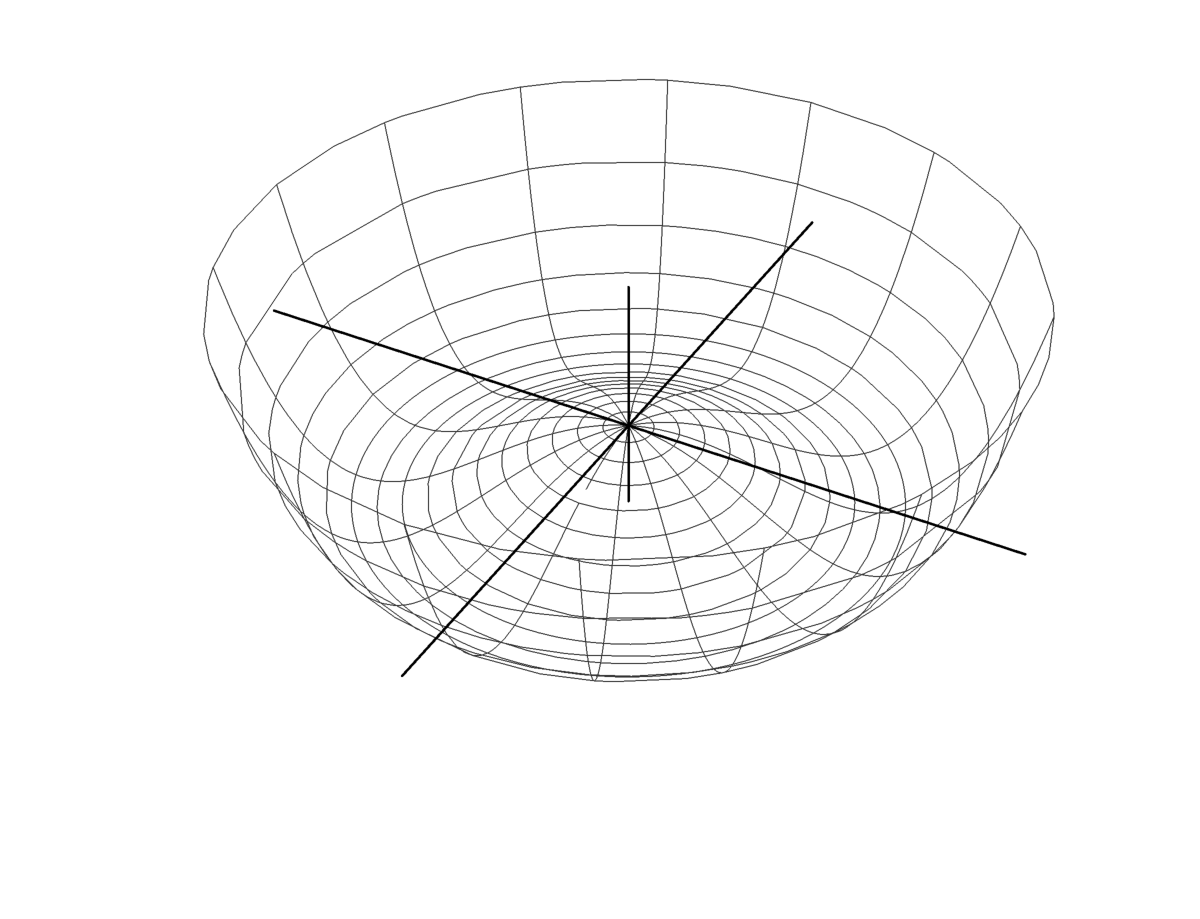
\includegraphics[width=3in]{3.pdf}
  \caption{对称性破缺后的势,$\sigma$场沿着径向涨落,$\pi^k$场沿着阱底切向方向涨落}
\end{figure}
\subsection{Goldstone定理}
连续对称性自发破缺时出现无质量的粒子叫做Goldstone定理. 例如线性$\sigma$模型中, 对于$N=1$时不存在连续对称性, 而$N>2$的情况下, 线性$\sigma$模型存在$\frac{N(N-1)}{2}$个连续对称性. 发生自发对称性破缺后残余的连续对称性有$\frac{(N-1)(N-2)}{2}$个, 对应的有$N-1$个$\pi$场.

Goldstone定理表述了对于每一个连续自发对称性破缺都必定包含一个无质量的粒子. 这个由于SSB导致的无质量粒子叫做Goldstone玻色子. 之前的线性$\sigma$模型中正好是这个定理的一个粒子. 现在我们在经典水平上证明这件事, 考虑一个包含若干场$\phi^a(x)$的拉氏量
\begin{equation*}
  \mathcal{L}=(\text{场的导数项})+V(\phi)
\end{equation*}
由于在$\phi_0^a$处$V$取到了极小值, 所以有
\begin{equation*}
  \left.\frac{\partial}{\partial\phi^a}V\right|_{\phi^a(x)=\phi_0^a}=0
\end{equation*}
在极小值处展开得到
\begin{equation*}
  V(\phi)=V(\phi_0)+\frac{1}{2}(\phi-\phi_0)^a(\frac{\partial^2}{\partial\phi^a\partial\phi^b}V)+\cdots
\end{equation*}
二次项系数为
\begin{equation*}
  \left(\frac{\partial^2}{\partial\phi^a\partial\phi^b}V\right)_{\phi_0}=m_{ab}^2
\end{equation*}
这是个对称矩阵,本征值给出了场的质量. 由于$\phi_0$是最小值, 这些本征值是非负的. 为了证明Goldstone定理, 我们必须展现出每一个不是$\phi_0$的连续对称性都产生一个零本征值.

一般的连续对称性有形式
\begin{equation*}
  \phi^a\rightarrow\phi^a+\alpha\Delta^a(\phi)
\end{equation*}
其中$\alpha$是一个无穷小参数, $\Delta^a$是所有$\phi$的一些函数. 对于经典场$\mathcal{L}$的一阶导数为$0$
\begin{equation*}
  V(\phi^a)=V(\phi^a+\alpha\Delta^a(\phi)),\quad \Delta^a(\phi)\frac{\partial}{\partial\phi^a}V(\phi)=0
\end{equation*}
上式同时对$\phi^b$求导, 然后令$\phi=\phi_0$
\begin{equation*}
  0=\left(\frac{\partial\Delta^a}{\partial\phi^b}\right)_{\phi_0}\left(\frac{\partial V}{\partial\phi^a}\right)_{\phi_0}+\Delta^a(\phi_0)\left(\frac{\partial^2}{\partial\phi^a\partial\phi^b}\right)_{\phi_0}
\end{equation*}
观察上式, 由于$\phi_0$是$V$的极小值, 第一项为$0$, 所以第二项也必须为$0$. 如果连续对称变换保持$\phi_0$不变, 有$\Delta^a(\phi_0)=0$. 若连续对称性导致$\phi_0$变化, 有$\Delta^a(\phi_0)\neq0$. 在这种情况下, $\left(\frac{\partial^2}{\partial\phi^a\partial\phi^b}V\right)_{\phi_0}$存在零本征值. 这样就在经典水平上证明了Goldstone定理.
\section{有限系统的自发对称性破缺}
之前的经典理论里我们使用了序参量$\langle\varphi(x)\rangle$来描述自发对称性$U(1)$的破缺, 量子理论中定义算符$W=e^{-i\hat{N}\theta}$来描述$U(1)$对称性. 由于
\begin{equation*}
  \begin{split}
     Wa(x)W^\dag&=e^{-iN\theta}ae^{iN\theta}=a(x)+[-iN\theta,a]+\frac{1}{2!}[-iN\theta,[-iN\theta,a]]+\cdots\\
       &=a(x)+i\theta a(x)+\frac{1}{2!}(i\theta)^2a(x)+\cdots=e^{i\theta}a(x)
  \end{split}
\end{equation*}
这里利用了$[N,a]=-a$
\end{document} 